% !TEX TS-program = xelatex

\documentclass[a4paper,twoside,11pt]{report} %openright
\newcommand{\documenttype}{Master Thesis}
\newcommand{\thesistitle}{Investigation of Deep Probibalistic Surrogate-models in Bayesian Optimization}
\newcommand{\thesissubtitle}{in Bayesian Optimization}

\newcommand{\thesisauthor}{Simon Saugmandsgaard Kruse} % Your name :) 
\newcommand{\studentnumber}{s164221}
\newcommand{\thedate}{June, 2022} % For example "June, 2019"

\newcommand{\department}{DTU Compute}
\newcommand{\departmentdescriber}{Section of Cognitive Systems}
\newcommand{\addressI}{Building 321}
\newcommand{\addressII}{2800 Kgs. Lyngby}
\newcommand{\departmentwebsite}{www.byg.dtu.dk}

\input{Setup/Preamble.tex}
\input{Setup/Settings.tex}
\usepackage{Setup/MoreSettings}

\begin{document}

\pagenumbering{roman}
\title{\thesistitle} 
\author{\thesisauthor} 
\date{\thedate} 

\begin{titlepage}

\newgeometry{left=11mm,right=11mm,top=50mm,bottom=0pt}
\pagecolor{frontbackcolor}
\color{\frontpagetextcolour}

\begin{flushleft}
{ % Thesis title (to change see Setup/Settings.tex) 
\Huge
\begin{tabular}{p{\linewidth}}
%\TitleFont{\thesistitle}   \\ 
\TitleFont{Investigation of Deep Probabilistic Surrogate-}\\
\TitleFont{models in Bayesian Optimization} \bigskip \\ 
%\titlefont{\thesissubtitle} \bigskip \\ 
{\huge Simon Saugmandsgaard Kruse}\\
{\LARGE \documenttype}\\
\end{tabular}
}
\end{flushleft} 

% DTU department (to change see Setup/Settings.tex) 
\begin{tikzpicture}[remember picture,overlay]
\node[anchor=north east, 
      xshift=-10mm, 
      yshift=-12mm] 
      at (current page.north east) 
      {
        \color{\frontpagetextcolour}
        \begin{tabular}{r} 
        \textbf{\department} \\ 
        \departmentdescriber
        \end{tabular}
      }; 
\end{tikzpicture}

% DTU logo
\begin{tikzpicture}[remember picture,overlay]
\node[anchor=north west, 
      xshift=8.9mm, 
      yshift=-8.3mm] 
     at (current page.north west) 
     {\includegraphics[width=14.75mm,keepaspectratio]{Pictures/Logos/\dtulogocolour_\targetcolourmodel.pdf}}; 
\end{tikzpicture}

% Cover photo
% \begin{tikzpicture}[remember picture,overlay]
% \node[anchor=south, % anchor is bottom of picture
%       xshift=0pt, 
%       yshift=-2.9mm] % shifting picture to actually be at the bottom of the page
%      at (current page.south) % placement at bottom of the page
%      {\includegraphics[height=18.9cm,keepaspectratio]{Pictures/BNN_posterior.pdf}};
% \end{tikzpicture}

\tikzset{every picture/.style={line width=0.75pt}} %set default line width to 0.75pt        

\begin{tikzpicture}[remember picture,overlay]
      \node[anchor=south, % anchor is bottom of picture
            xshift=-15mm, 
            yshift=30mm]
            at (current page.south){
            %\path (0,310); %set diagram left start at 0, and has height of 310
            \resizebox{1.34\textwidth}{!}{%
            \begin{tikzpicture}[x=0.55pt,y=1.25pt,yscale=-1,xscale=1]
              %Curve Lines [id:da9880396283111128] 
              \draw    (-3,149) .. controls (37,119) and (631,152) .. (671,122) ;
              %Shape: Free Drawing [id:dp07450350989511567] 
              \draw  [color={rgb, 255:red, 0; green, 0; blue, 0 }  ,draw opacity=1 ][line width=3] [line join = round][line cap = round] (1,217) .. controls (9.22,217) and (16.92,223.69) .. (25,226) .. controls (41.54,230.73) and (74.95,221.05) .. (87,209) .. controls (105.26,190.74) and (119.38,166.92) .. (134,145) .. controls (139.73,136.41) and (145.18,124.73) .. (154,119) .. controls (162.38,113.56) and (171.87,110.06) .. (181,106) .. controls (194.08,100.19) and (206.2,94.54) .. (221,94) .. controls (252.1,92.87) and (283.1,92.65) .. (313,102) .. controls (325.49,105.9) and (359.46,131.87) .. (369,138) .. controls (378.91,144.37) and (389.67,149.33) .. (400,155) .. controls (427.23,169.93) and (448.29,187.48) .. (479,198) .. controls (503.38,206.35) and (531.3,202.09) .. (556,199) .. controls (595.29,194.09) and (632.75,185.23) .. (672,184) ;
              %Shape: Free Drawing [id:dp6323192319779791] 
              \draw  [line width=3] [line join = round][line cap = round] (-5.92,100) .. controls (-2.51,100) and (6.86,94.78) .. (9.33,96) .. controls (17.1,99.82) and (23.07,109.05) .. (32.7,108) .. controls (40.32,107.17) and (44.09,97.82) .. (48.97,92) .. controls (49.4,91.49) and (48.97,89.33) .. (48.97,90) .. controls (48.97,102.37) and (56.01,118.15) .. (60.15,129) .. controls (60.26,129.31) and (76.41,110) .. (76.41,110) .. controls (76.41,110) and (80.82,124.16) .. (81.49,127) .. controls (84.55,140.04) and (89.44,152.65) .. (94.7,165) .. controls (95.54,166.97) and (97.67,161.84) .. (98.77,160) .. controls (101.4,155.57) and (111.47,139.87) .. (116.05,141) .. controls (119.15,141.76) and (119.5,146.29) .. (121.13,149) .. controls (129.92,163.6) and (136.07,175.33) .. (149.59,185) .. controls (158.99,191.73) and (162.41,187.67) .. (168.9,182) .. controls (171.5,179.72) and (175.69,174.47) .. (178.04,177) .. controls (190.74,190.63) and (200.54,205.13) .. (218.7,212) .. controls (224,214.01) and (231.73,204.77) .. (233.94,203) .. controls (246.38,193.06) and (257.18,181.7) .. (260.37,166) .. controls (260.8,163.91) and (262.66,169.78) .. (264.44,171) .. controls (269.67,174.61) and (274.92,178.31) .. (280.7,181) .. controls (292.33,186.42) and (312.48,194.15) .. (326.43,189) .. controls (333.1,186.54) and (332.01,176.06) .. (335.58,170) .. controls (337.02,167.55) and (339.98,166.28) .. (341.68,164) .. controls (343.92,160.99) and (346.76,154) .. (346.76,154) .. controls (346.76,154) and (350.46,159.64) .. (352.86,162) .. controls (358.69,167.74) and (366.25,173.74) .. (375.22,173) .. controls (391.02,171.7) and (401.03,149.88) .. (407.74,139) .. controls (411.3,133.23) and (415.86,128.04) .. (418.92,122) .. controls (420.99,117.94) and (421.34,113.23) .. (422.99,109) .. controls (425.17,103.42) and (424.76,112.05) .. (432.14,117) .. controls (437.52,120.61) and (443.28,123.83) .. (449.42,126) .. controls (457.24,128.77) and (473.31,123.11) .. (479.91,120) .. controls (490.71,114.92) and (506.25,108.08) .. (514.46,100) .. controls (519.38,95.16) and (524.15,90.18) .. (528.69,85) .. controls (530.02,83.49) and (532.26,77.7) .. (535.81,77) .. controls (543.28,75.53) and (543.2,83.93) .. (548,90) .. controls (553.94,97.51) and (566.06,101.59) .. (575.44,98) .. controls (588.4,93.04) and (603.28,84.05) .. (615.08,77) .. controls (619.26,74.51) and (623.3,71.79) .. (627.28,69) .. controls (628.06,68.45) and (628.35,67) .. (629.31,67) .. controls (630.84,67) and (638.51,73.56) .. (639.48,74) .. controls (642.42,75.35) and (653.36,77.33) .. (656.75,80) .. controls (659.19,81.92) and (659.73,87) .. (662.85,87) .. controls (664.25,87) and (665.56,86.33) .. (666.92,86) ;
            \end{tikzpicture}
            }%  
            };
      \end{tikzpicture}


\end{titlepage}

\pagecolor{white}
\newgeometry{top=2.81cm, bottom=2.75cm, outer=2.5cm, inner=3.5cm}
\pagestyle{empty}
\cleardoublepage 
\thispagestyle{empty}
\setcounter{page}{1}
\vspace*{\fill}

\textbf{\thesistitle} \newline
\thesissubtitle

\smallskip

\documenttype \newline
\thedate

\smallskip

By \newline
\thesisauthor

\bigskip

\begin{tabularx}{\textwidth}{@{}lX@{}}
    Copyright: & Reproduction of this publication in whole or in part must include the customary bibliographic citation, including author attribution, report title, etc. \\
    Published by: & DTU, \departmentdescriber, \addressI, \addressII ~Denmark  \\
\end{tabularx}



\clearpage 
\pagestyle{main}
\section*{Approval}
\addcontentsline{toc}{section}{Preface}
This master thesis was prepared at the Section of Cognitive Systems at the Technical University of Denmark in
fulfillment of the requirements of the degree Master of Science in Engineering, MSc Eng, in Mathematical Modeling and Computation.

%The work was carried out in the spring of 2022 and project covers a work load of 30 ects point. 
\vfill

\begin{center}
\namesigdate{\thesisauthor~-~\studentnumber}
\end{center}

\vfill


\clearpage 
\section*{Abstract}
\addcontentsline{toc}{section}{Abstract}
% Abstract
%  1. Motivation. Why do we care?
Bayesian optimization (BO) is the leading methodology in sample-efficient optimization and
widely used in hyperparameter tuning in machine learning and deep learning. 

%  2. Problem formulation. What problem will we solve?
%     2.b. Current state. What have others done, and why is that not enough?
From a decision theoretical standpoint, assuming the probabilistic surrogate model to be correct
is crucial for the correct decision. We will investigate if other surrogate models could be better
than the BO default: Gaussian process (GP). 

%  3. Approach. What is our big idea? How did we solve it?
%     3.a. Analysis and experiments. What research did we do?
This thesis investigates surrogate models such as Mixture regression and Bayesian neural
networks(BNN) and compares them against GP. To have a good chance of analyzing the
models, the focus is first to understand and present the theory and second to apply the
models in a BO setting. 

%  4. Results. What is the answer?
%  5. Conclusions. What are the implications?
After understanding and presenting the different surrogate models and corresponding inference
methods. Tests were conducted on four self-made 1D Problems and a commonly used benchmarking problem
set. The mixture and BNN regression results were promising for classes of problems with
discontinuities and multimodality, and the GP was found best for most tests. All surrogate models
were Gaussian approximated in the BO tests, especially this compromisation of the mixture regression models
sparks even more promise for their positive results.tests



\clearpage 

\section*{Acknowledgements and background}
\addcontentsline{toc}{section}{Acknowledgements}
%\textbf{\thesisauthor}, MSc Civil Engineering, DTU

This thesis is the culmination of the last years excitement about Bayesian statistics and Bayesian
computing. I found probability theory very hard when I was introduced to it in 2017, and I only knew
statistics like p-values and t-tests, and I was tired of looking at plots without really understanding
why they made sense. Not satisfied with, from my point of view the "fluffy handwaving"- statistics - I
avoided many of the statistics courses and found happiness in the hardcore proof-founded courses such as
real analysis, abstract algebra, and numerical optimization. However, since machine learning was my big
passion and the reason why I chose to study applied mathematics, at some point I was introduced to
probabilistic machine learning, using Bayesian statistics. Learning about Bayesian statistics
flipped around my view on statistics for good. The concept of a probabilistic model came very late and
was a game-changer. I had a very good course at TU Delft, \textit{statistical inference} - a hardcore
proof-founded course, which helped my frustrations of not truly understanding what p-values and
statistical tests are.

%Even though we never really spoke, I need to thank Professor Frank van der Meulen for his 
% Tommy Sonne Alstrøm was my tutor in 2017, his advice to me of focusing on the hard mathematics courses
% gave me encouragement to take the hard math courses, with no obvious relevance to the world. Today
% I consider real and functional analysis courses the most important courses for maturing my
% mathematical mindset. I need to thank my two supervisors <..>

% This thesis is also a natural extension of my bachelor thesis in numerical optimization
% \textit{Trust-region methods for structural optimization}, with Martin Skovgaard and.. This thesis
% is all that I wanted, being the combination between  


\cleardoublepage 
\tableofcontents
\cleardoublepage 

%%%%%%%%%%%%%%%%%%%%%%%%%%%%%%%%%%%%%%%%%%%%%%%%%%%%%%%
\pagenumbering{arabic}
\chapter{Introduction}
% Introduction section
%  1. Introduction.
%  2. Background and setting. 
%  3. Identification of problem
%  4. Purpose Statement. 
%  5. Objectives or research questions
%  6. Assumptions. Limitations. Definition of terms
%  7. Significance of the study.

% Introduction section (from unsw.edu.au)
% Move A: establish your territory (say what the topic is about)
%   1.  state the general topic and give some background
%   2.  provide a review of the literature related to the topic
%   3.  define the terms and scope of the topic
Optimization plays an important part in our everyday life, science development, and product design.
What transportation should you choose to get fast from A to B? What songs should
land on your playlist? and what is the optimal bridge construction? In general, optimization is the
art of choosing the best decision. Often we can quantify how good a decision is: A bus takes 20 min,
a car takes 15 min to go from A to B, How would you rate the song?
This bridge construction costs 10 million. If it is possible to come up with a quantification of how good
a decision is in terms of a real number, then we can define is a \textit{mathematical optimization problem}: 
$$\min_{x\in \mathcal{X}} f(x)$$ where the functional $f: \mathcal{X} \rightarrow \mathbb{R}$ is
called the objective function and $\mathcal{X}$ is the set of possible decisions (or decisions you consider).
The optimization problem is now in the domain of cold numbers and here many algorithms have been developed
to find the minimum of the function $f(\cdot)$. Note that we throughout this thesis refer to
optimization as minimizing a cost function - this is equivalent to maximizing the negated function
$\max_{x\in \mathcal{X}} f(x) = \min_{x\in \mathcal{X}} -f(x)$.  

Evaluation of the objective function can be cheap e.g. if it just requires
summing and multiplying numbers or highly expensive if it involves human rating or large simulation
and physical experiments. Bayesian optimization is a preferred <ref> framework for optimization of
the expensive objective functions. And is also referred to as \textit{sample efficient}
optimization.

Bayesian optimization is a probabilistic surrogate-based optimization methodology: Assuming some samples from a
highly expensive objective a cheap (surrogate) function is used to fit the samples. The next sample
is found by minimizing the surrogate and the process is repeated. Bayesian optimization seeks to
enhance this procedure with probability theory, where the surrogate function becomes a probabilistic
regression model. The most common choice is a Gaussian Process, as it encapsulates the uncertainty very well,
but also because its inference procedure (computing answers to probability queries like $p(y|x)$) is exact.

% Move B: establish a niche (show why there needs to be further research on your topic)
%   4.  outline the current situation
%   5.  evaluate the current situation (advantages/ disadvantages) and identify the gap

\section{Weakness of GPs}
Using GP with isotropic kernel function, have continous sample paths, 
which might be undesired . 


Even though GP has proven good for many cases, there will be problems where the assumptions do not hold. 
The assumptions of a GP are essential that the objective function can be described as a GP.
The nature of a GP is highly dependent on the choice of its kernel and the parameters chosen in that kernel. 
Another reason for the popularity of the GP is the closed-form inference and giving a closed-form of the 
expected improvement acquisition function. 

$$p(y|x, \mathcal{D}) = GP(f(x)|\mu(x), \kappa(x,x)) \implies x_{next} = \arg\max_x \sigma_x [u\Phi(u)+ \phi(u)]$$


% Move C: introduce the current research (make hypotheses; state the research questions)
%   6.  identify the importance of the proposed research
%   7.  state the research problem/ questions
%   8.  state the research aims and/or research objectives
%   9.  state the hypotheses
%   10. outline the order of information in the thesis
%   11. outline the methodology

\section{No free lunch and surrogate reseach}

<No free lunch theorem for optimization>, establish some questions on why there is no best method.
And a burning research problem is if it is possible to use a different surrogate model than the GP. 
And whether or not they in general performs better? What assumptions underlie the problem. 
The assumption for GP regression is that the objective function follows a Gaussian process, whereas
we assume it follows a random forest or neural network. These are assumptions that yields, consideration:
Is this a good assumption? Bayesian NNs are very expressive. 

Bayesian multivariate adaptive
regression splines (BMARS)30,31 and Bayesian additive regression
trees (BART)32 a
shows superior when f, requires more flexible model. 

surrogates: 
\begin{itemize}
    \item GP
    \item BNN
    \item Random forest
    \item SPN
    \item Kernel estimator
\end{itemize}

Within Bayesian surrogate model, there has been research on using random forest or Bayesian neural 
networks. The PhD thesis "Sample-efficient Optimization Using Neural Networks" from 2020 \cite{PhDthesis}
showcases empirically that using Bayesian neural networks as surrogate models performed better,
or at least comparable to GPs on a wide number of problems. The performance difference was more
clear for high-dimensional problems. 

While most alternative method are investigated due to the expensive inference time for GPs, 
this thesis investigates alternative surrogates as a method of 

Another regression model not seen much in the literature is Gaussian mixture regression, which
is modeling the joint distribution between x and y, and using the conditional distribution $p(y|x)$
as the regression model, which is provided exactly. 

Research problem/question:
\begin{itemize}
    \item Which type of optimization problem is a GP not a good choice?
\end{itemize}

\begin{figure}[H]%
    \centering
    {\includegraphics[width=0.46\textwidth]{Pictures/GP_vs_BNN1.pdf} }%
    \qquad
   {\includegraphics[width=0.46\textwidth]{Pictures/GP_vs_BNN2.pdf} }%
    \caption{Example where The discontinuerity makes the GP overreact to all other 
    uncertainties}%
    \label{fig:example}%
\end{figure}


Research aims:
As a new model Sum product networks has become a promissing method. Shown to be the most 
general probabilistic model that allows for exact inference! <ref>. It has relation to 
neural networks (but with the limit of not being too deep) and Bayesian networks, and provides
a framework for learning and inference in deep probabilistic models. As nice as it sounds
the project will investigate what SPNs are and how it can be used as a surrogate models. 

As we will see later SPNs are just exponentially large mixture models, and therefore 
it is interesting to investigate Kernel estimators.

state the hypotheses
\begin{itemize}
    \item Will an SPN work as a surrogate model?
    \item We can find problems where GPs fails to establish good predictions. 
    \item BNN might work as well as GPs
\end{itemize}

%   10. outline the order of information in the thesis
%   11. outline the methodology


\section{Old intro}
%<What is optimization>
Optimization plays an important part in our everyday life, science development, and product design.
What different transportation should you choose to get fast from A to B, what songs should
land on your playlist, and what is the optimal bridge construction. Mathematical optimization problems 
are all problems in the form, 
$$\min_{x\in \mathcal{X}} f(x)$$ where $f: \mathcal{X} \rightarrow \mathcal{R}$ is a functional. I.e
if it is possible to set up an objective function. e.g. what is the cost of the bridge given a
specific design, or how pleasant you think some music, and some constraints such that you keep in
the domain of interest. Evaluation of the objective function can be cheap e.g. if it just requires
summing and multiplying numbers or highly expensive if it involves human rating or large simulation
and physical experiments. Bayesian optimization is a preferred <ref> framework for optimization of
the expensive objective functions. And is also referred to as \textit{sample efficient}
optimization. 
%<Why Bayesian optimization?>

Bayesian optimization is a probabilistic surrogate-based optimization: Assuming some samples from a
highly expensive objective a cheap (surrogate) function is used to fit the samples. The next sample
is found by minimizing the surrogate and the process is repeated. Bayesian optimization seeks to
enhance this procedure with probability theory, where the surrogate function becomes a probabilistic
regression model. The most common choice is a Gaussian Process, as it encapsulates the uncertainty very well,
but also because its inference procedure (computing answers to probability queries like $p(y|x)$) is exact.

Even though GP has proven good for many cases, there will be problems where the assumptions do not hold. 
The assumptions of a GP are essential that the objective function can be described as a GP.
The nature of a GP is highly dependent on the choice of its kernel and the parameters chosen in that kernel. 
Another reason for the popularity of the GP is the closed-form inference and giving a closed-form of the 
expected improvement aqurisition function. 

The PhD thesis "Sample-efficient Optimization Using Neural Networks" from 2020 \cite{PhDthesis}
showcases empirically that using Bayesian neural networks as surrogate models performed better,
or at least comparable to GPs on a wide number of problems. The performance difference was more
clear for high-dimensional problems. 

This master thesis project will investigate surrogate models alternative to Gaussian processes in
Bayesian optimization. Firstly by examining what types of problems a GP surrogate is not a good
choice for and where Bayesian neural nets (BNN) surrogates can have an advantage (inspiration found in
this 2020 thesis [1]). Secondly by looking at sum-product networks (SPN) as novel surrogate models.
An SPN is - similarly to a BNN - a deep probabilistic model and still expressive but with tractable
inference, which potentially could lead to advantages over BNNs. 

%#<Short overview of types of surrogate models>

<Make a figure of how the parts are all connected>

\section{notation}
Throughout this thesis we will be using Bayesian notation, i.e. $p(x) := P(X=x)$ is 
the probability density function of the random variable $X$ evaluated in $x$. 
and $p(y|x) := P(Y=y|X=x)$ or $p(y|x) := P(Y|X=x)$.

And writing $p(y^2|x)$ means $P(Y^2=y^2|X=x)$ and \textbf{not} $P(Y=y^2|X=x)$

\section{related work}
This thesis is 
<BAHAMIANN>

<DNGO>
Focus on the inference time of GP scales cubic, which is not appropriate for
parallel BayesOpt. 
Experiments on 6dim Hartmann function. 

<Arayns paper.>
Conclusions..!?

Already developed alternative surrogate models has been found in the litterateur. The last presented
surrogate model, SPN, is to our knowledge not in any published work. More models might still be
added to the list. 

\subsubsection*{DNGO}
Deep Networks for Global Optimization (DNGO) is presented in the paper 2015 paper "Scalable Bayesian
Optimization Using Deep Neural Networks"\cite{snoek2015scalable}. The surrogate model is a neural
network, where only the last layer is probabilistic, this leads to Bayesian regression and very fast
inference.  

\subsubsection*{BOHAMIANN}
\textbf{B}ayesian \textbf{O}ptimization with \textbf{Hami}ltonian Monte Carlo \textbf{A}rtificial
\textbf{N}eural \textbf{N}etworks (BOHAMIANN) is presented in the 2016 paper "Bayesian Optimization
with Robust Bayesian Neural Networks"\cite{NIPS2016_a96d3afe}. This is a fully Bayesian Neural
Network trained using adaptive Hamiltonian MCMC. 
%\subfile{Text/til_mikkel.tex}
\cleardoublepage

\section{Optimization methodology}
Given an objective function $f: \mathcal{X} \rightarrow \mathbb{R}$, where the domain
$\mathcal{X}$ could be a subset of $\mathbb{R}^n$,
optimization is a methodology which seeks to find an optimal point, $x^*$, and value
$f^* = f(x)$, given as
\begin{align}\label{OPT}
    x^* \in \argmin_{x \in \mathcal{X}} f(x) \hspace{1cm} f^* = \min_{x \in \mathcal{X}} f(x) = f(x^*).
\end{align}
Note that the above formulation is a minimization problem, which is equivalent to a
maximization problem maximizing $-f(\cdot)$. Throughout this thesis, we choose to only work
with a minimization problem. 
Solving this problem (close to) exact is often intractable except for rare cases e.g. if $f$ is 
convex and analytically directly solvable or the domain of $f$ is very limited. The following example
with linear least squares is an example of such a problem. 

\begin{testexample}[Direct solution method]
    The unconstrained linear least squares, $$\min_{x\in \mathbb{R}^n} f(x) := ||Ax-b||_2^2$$
    where $A \in \mathbb{R}^{m\times n}$ and $b \in \mathbb{R}^m$, is a convex problem,
    i.e. finding $x^*$ such that $\nabla f(x^*) = 0$ is equivalent to finding the solution
    to the problem. Assuming $A^TA$ is invertable, linear least squares can be solved
    directly by the normal equations, 
    $$\nabla f(x) = 2A^TAx + 2b^TA = 0 \hspace{0.5cm} \Leftrightarrow \hspace{0.5cm} x^* = (A^TA)^{-1} A^Tb$$
\end{testexample}

Most optimization problems are non-convex with multiple local minima. And even if the gradient is
given analytically, the solution is still found among a potentially infinitely large set of
stationary points ($\nabla f(x) = 0$) and boundary points ($x \in \partial \mathcal{X}$) - this
might be tedious or impossible. Therefore, when the problem is not directly solvable, mathematical optimization
takes an indirect approach: Design a sequence of experiments that reveal information about the
objective function. This information can hopefully lead us to the solution of \eqref{OPT}. This
general way of sequentially solving is presented in the book Bayesian Optimization by Roman Garnett
\cite{bayesoptbook} and presented here as Algorithm \ref{algOPT}. 

\begin{algorithm}
\caption{Sequencial Optimization \cite{bayesoptbook} }\label{algOPT}
\begin{algorithmic}
\State \textbf{Input:} Initial dataset $\mathcal{D}$  \Comment{can be empty}
\While{Temination is not reached}
    \State $x \gets \text{policy}(\mathcal{D})$ \Comment{select next observation location}
    \State $y \gets \text{observe}(x)$ \Comment{observe objective function at chosen location}
    \State $\mathcal{D} \gets \mathcal{D} \cup \{(x,y)\} $ \Comment{update dataset}
\EndWhile
\State $\textbf{return: } \mathcal{D}$
\end{algorithmic}
\end{algorithm}

Given data points in the \textit{optimization landscape}\footnote{"Optimization landscape" defined
as the joint set of points in the domain and the objective function evaluated in the points, i.e.
$\{(x,f(x))\in \mathcal{X} \times \mathbb{R}| x \in \mathcal{X}\}$} a policy selects a location $x
\in \mathcal{X}$ where we make our next observation. Policies can be deterministic or probabilistic;
examples of each type could be grid search and random search. The next observation provides us a $y$
value, which combined with $x$ is included in the available data $\mathcal{D}$. Finally, a stopping
criterion decides whether to repeat or terminate the procedure. We will now present how different
examples of well-known optimization routines fits into Algorithm \eqref{algOPT}.


\begin{testexample}[Grid search]
    In grid search values along each dimention in $\mathcal{X}$ is seleced and combined with each
    other, which thereby defines a parrellel grid in the optimization domain $\mathcal{X}$. All
    grid points are ordered and systematically selected. In the context of algorhtim \ref{algOPT} we define
    the grid search policy as 
    $$\text{policy}_{GS}(\mathcal{D}) = x_{|\mathcal{D}|+1}$$
    assuming $x_1,x_2, \dots, x_{m} \in \mathcal{X}$ are the ordered grid points and the size of the obtained 
    data is $|\mathcal{D}|$. Termination will happen when $|\mathcal{D}| = m$.
\end{testexample}
\begin{testexample}[Random search]
    In random search a point is randomly drawn from a uniform distribution supported over the domain
    space $\mathcal{X}$, 
    $$\text{policy}_{RS}(\mathcal{D}) = x, \hspace{0.5cm} x \sim Unif(\mathcal{X})$$
\end{testexample}
\begin{testexample}[Gradient descent]
    Gradient descent (GD) is the most simple gradient-based optimization approach. The gradient of a
    continuous function points in the most ascending direction at the location it is evaluated. GD
    iteratively minimize the objective function by taking steps using opposite gradient direction,
    i.e. the most descending direction, weighted with a stepsize $\eta$. This yields the policy:
    $$\text{policy}_{GD}(\mathcal{D}) = x_n - \eta \nabla f(x_n)$$
    where we, for a brief moment, in Algorithm \eqref{algOPT} modify $y$ to be a vector since the observation 
    is given as:
    $$\text{observe}_{GD}(x) = [f(x), \nabla f(x)]$$
\end{testexample}

\subsection{Sample-efficient optimization}
Note that grid search, random search, and gradient descent are policies that entirely ignore the
available data. Ignoring potentially valuable information is a shame if the objective function is
expensive to evaluate. And indeed, improvements of the gradient descent algorithm, such as momentum
and quasi-newton methods, indirectly remember and exploit obtained data, $\mathcal{D}$. They are
examples of so-called \textit{sample-efficient} solvers since they need fewer $y$-samples to
minimize $f(\cdot)$. Choosing a more sample-efficient solver ultimately costs extra time/energy, due
to the extra work of storing and exploiting the collected information for every iteration. In the
end, solving the optimization problem can be divided into the following components, 

\begin{itemize}[noitemsep]
    \item $N_{\text{iter}}$: The number of iterations to reach an acceptable solution. This number depends on the
    solver. If $N_{\text{iter}}$ is relatively small, the solver is called sample-efficient. 
    \item $C_{\text{policy}}$: The solvers cost per iteration, i.e. what is the cost of calculating
    $\text{policy}(\mathcal{D})$, where cost is typically in terms of time and power usage. 
    \item $C_{\text{observe}}$: Cost per evaluation of the objective function, i.e. the cost of $\text{observe(x)}$,
    which can be in terms of power consumption, human resources, simulation time etc.
\end{itemize}
Assuming same cost pr iterations and for all evaluations, the total optimization cost, $C_{\text{total}}$, is given as 
$$C_{\text{total}} = N_{\text{iter}} \cdot \left[ C_{\text{policy}} + C_{\text{observe}}\right]$$

A sample efficient solver has a large $C_{\text{policy}}$ but a small $N_{\text{iter}}$, whereas a
simple optimization scheme like random search has a very small $C_{\text{policy}}$ but a large
$N_{\text{iter}}$. Choosing the right optimization solver depends highly on $C_{\text{observe}}$.
For small $C_{\text{observe}}$ it is favorable to find a good trade-off between $N_{\text{iter}}$
and $C_{\text{policy}}$: In deep learning the solver Adam is very popular, due to its cheap
but advanced policy \cite{Adam}. This project deals with a dominating observation cost, i.e. the cost of the policy is assumed
neglectable $C_{\text{observe}}>>C_{\text{policy}}$. So focus is not on finding a cheap policy but rather
on improving the number of iterations to reach the minima $N_{\text{iter}}$.

\begin{testexample}[Surrogate-based optimization]
    %<SVR> <Radial Basis function> <Polynomal model/respons surface>
    In surrogate-based optimization all available data is fitted by a cheap-to-evaluate
    approximation to the objective function - this approximation is called a \textit{surrogate
    model}, $f_{\text{sur}}(x)$. Examples of surrogate models could be a radial basis function or a
    support vector regressor \cite{deterministicsurrogatemodels}. The next point is chosen as the point where the surrogate model is
    minimized. 
    $$\text{policy}_{\text{sur}}(\mathcal{D}) = \min_x f_{\text{sur}}(x)$$
    where $f_{\text{sur}}(x) \approx f(x)$ for $x$ close to the data $\mathcal{D}$. And we hope the approximation
    holds for $x$ far away from the the data.
\end{testexample}
\begin{figure}[H]%
    \centering
    {\includegraphics[width=0.46\textwidth]{Pictures/BO_vs_Grid2.eps} }%
    \qquad
   {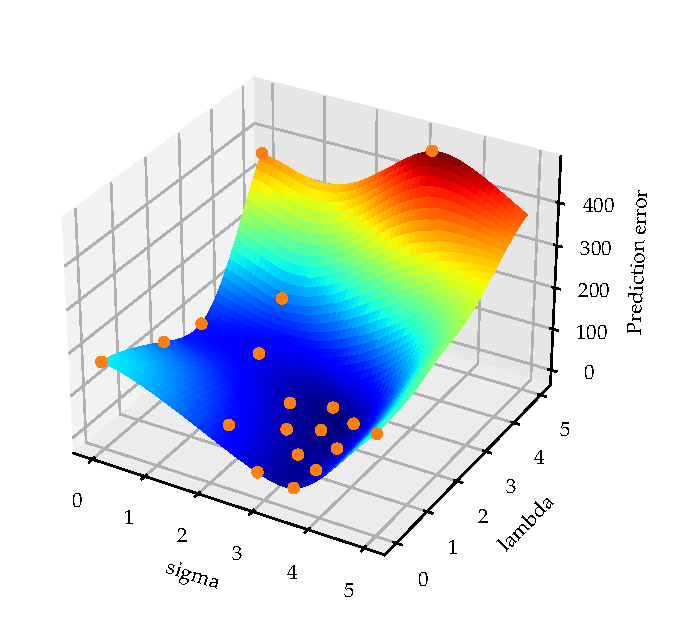
\includegraphics[width=0.46\textwidth]{Pictures/BO_vs_Grid1.eps} }%
    \caption{Example of an optimization task tuning a parameterised regression model with parameters
    $\lambda$ and $\sigma$, on a test set, i.e. minimization of prediction error. We see the first
    23 evaluations out of 100 in grid search vs 23 evaluations using a sample-efficient solver (Bayesian
    optimization). This illustrates the idea of a sample-efficient solver}%
    \label{fig:example}%
\end{figure}

\subsection{Exploitation and exploration}
The balance between an optimization procedure's local/exploitation and global/exploration elements
is key to its performance (statement in thesis \cite{PhDthesis} ok?). Explained here:
\begin{enumerate}
    \item Local element: Exploiting the obtained information $\mathcal{D}$ to find the best point
    \item Global element: Obtaining new information about the characteristics of the objective
    function.
\end{enumerate}
Essentially, the only explorative phase of the deterministic surrogate optimization is the first
initial samples from the objective, i.e. when creating the initial $\mathcal{D}$. If done poorly,
the optimization might get stuck in a local minimum. This is a consequence of their nonexisting
ability to express uncertainty about the objective function. Deterministic surrogate models do not
pay attention to less-explored regions, which is the essential characteristic of a global
optimization method \cite{GlobalOptimization}. 

Bayesian formalism is a powerful and sound tool for incorporating uncertainty into the surrogate
model. Prior to any observed data, we can easily integrate our beliefs about the distribution of
the objective function. When observing data, the likelihood and prior collaborate to create a
predictive (posterior) distribution, $p(y|x,\mathcal{D})$. The next location $x$ to explore is now
determined with a theoretically motivated policy (acquisition function) which might balance the
exploitation and exploration tradeoff. 

Moreover, Bayesian optimization (or \textit{probabilistic} surrogate-based optimization) is motivated by
its ability to deal with noisy objective functions. 


\subsection{Noisy objective functions}
Many optimization algorithms assume \textit{exact} evaluations of the objective function. However,
this assumption is often wrong, especially for objective functions with real-life experiments,
imperfect simulations, human interaction where measurement noise is well known. A potentially noisy
objective function is the main reason why we in Algorithm \eqref{algOPT} use the terminology
$\text{observe}(x)$ and not just \textit{evaluate }$f(x)$.

The observation model is typically noisy and described as
$$y = f(x)+\epsilon$$ where $\epsilon$ is the measurement error, this is
typically assumed to be Gaussian with zero mean and a variance
$\sigma^2$ (which could depend on $x$ in a heteroskedastic setting) and implies a Gaussian observation model, 
$$p(y|f(x),\sigma^2) = \mathcal{N}(y|f(x),\sigma^2)$$ 

% (note from now on we define $\phi := f(x)$ in order to avoid confusion and a extra set of paranteses)
% $$p(y|x,\phi,\sigma) = \mathcal{N}(y;\phi,\sigma^2)$$ 
\begin{note2}["Sampling" from objective function]
    The terminology \textit{to sample} is refering to a probabilistic observation model. Formally, we
    can extend this model to deal with noiseless observations as well, simply by setting
    $\sigma = 0$ and letting the model colaps into a Direct delta distribution, $p(y|f(x)) =
    \mathcal{\delta}(y-f(x))$, i.e. all probability mass for $y$ is on the value $f(x)$ giving the
    observation sample $y = f(x)$. 
\end{note2}

% \begin{note}
%     \textbf{"Sampling" from objective function} 
%     The terminology \textit{to sample} is refering to a probabilistic observation model. Formally, we
%     can extend this model to deal with noiseless observations as well, simply by setting
%     $\sigma = 0$ and letting the model colaps into a Direct delta distribution, $p(y|f(x)) =
%     \mathcal{\delta}(y-f(x))$, i.e. all probability mass for $y$ is on the value $f(x)$ giving the
%     observation sample $y = f(x)$. 
% \end{note}

Bayesian optimization or probabilistic surrogate-based optimization deals with both noiseless and noisy objective functions,
as it defines a Bayesian regression model over the observations.

% \begin{figure}[h]
%     \centering
%     \includegraphics[width=0.9\textwidth]{Pictures/BO_vs_Grid2.eps}
%     \caption{Hyper parameter tuning of a model $M(\lambda, \sigma)$, 
%     35 evaluation in grid search vs 39 evaluations using Bayesian optimization}
%     \label{optimhist}
% \end{figure}

\begin{testexample}[Bayesian Optimization]
    Bayesian optimization is a \textit{probabilistic} surrogate-based optimization
    methodology. Here a cheap probabilistic regression model $p(y|x)$ is fitted to the
    the observations $\mathcal{D}$ and in contrast to (deterministic) surrogate-based
    optimization, it is not possible right away to find the minima in the cheap
    surrogate model; first, we need to interpret the meaning of minima in a probabilistic
    regression model. This interpretation is done through a so-called acquisition
    function (more about this later). The policy is as following,
    $$\text{policy}_{BO}(\mathcal{D}) = \max_x AQ(p(y|x,\mathcal{D}))$$

    \begin{figure}[H]
        \begin{minipage}[c]{0.67\textwidth}
          \includegraphics[width=\textwidth]{Pictures/BO_example.pdf}
        \end{minipage}\hfill
        \begin{minipage}[c]{0.3\textwidth}
          \caption{Top: Bayesian regression model (Gaussian Process) is fitted to the observed data,
          which are sampled from the underlying objective (black sin-function). Bottom: The expected improvement
          \textit{acquisition function} is maximied at the orange arrow, i.e. the location of the
          next sample.  $\text{policy}_{BO}(\mathcal{D}) = 26,06$} \label{BO_example}
        \end{minipage}
    \end{figure}
\end{testexample}


% \begin{tcolorbox}[
%     sharp corners,
%     boxrule=0mm,
%     enhanced,
%     borderline west={4pt}{-2pt}{darkred},
%     borderline north={1pt}{0pt}{darkred},
%     borderline south={1pt}{0pt}{darkred},
%     borderline east={1pt}{0pt}{darkred},
%     %colframe=darkred!0,
%     %colback=darkred!10,
%     %coltitle=darkred,
%     %boxsep=3pt,left=4pt,right=4pt,top=2pt,bottom=2pt
% ]
% { \textcolor{darkred}{\textbf{Example: Bayesian Optimization}}}\\
%     Bayesian optimization is a \textit{probabilistic} surrogate-based optimization
%     methodology. Here a cheap probabilistic regression model $p(y|x)$ is fitted to the
%     the observations $\mathcal{D}$ and in contrast to (deterministic) surrogate-based
%     optimization, it is not possible right away to find the minima in the cheap
%     surrogate model; first, we need to interpret the meaning of minima in a probabilistic
%     regression model. This interpretation is done through a so-called acquisition
%     function (more about this later). The policy is as following,
%     $$\text{policy}_{BO}(\mathcal{D}) = \max_x AQ(p(y|x,\mathcal{D}))$$

%     \begin{figure}[H]
%         \begin{minipage}[c]{0.67\textwidth}
%           \includegraphics[width=\textwidth]{Pictures/Test1Gaussian_Process_-_sklearn000.pdf}
%         \end{minipage}\hfill
%         \begin{minipage}[c]{0.3\textwidth}
%           \caption{Top: Bayesian regression model (Gaussian Process) is fitted to the observed data,
%           which are sampled from the underlying black objective. Bottom: The expected improvement
%           \textit{acquisition function} is maximied at the orange arrow, i.e. the location of the
%           next sample.  $\text{policy}_{BO}(\mathcal{D}) = -79,27$} \label{fig:03-03}
%         \end{minipage}
%     \end{figure}
   
% \end{tcolorbox}


% \begin{algorithm}[H]
%     \caption{Bayesian Optimization}
%     \begin{algorithmic}
%     \State \textbf{Input:} Initial dataset $\mathcal{D}$, Bayesian regression model.
%     \While{Temination is not reached}
%         \State Fit Bayesian regression model: $$p(y|x,\mathcal{D}) = \int p(y|x,\theta)p(\theta|\mathcal{D})d\theta$$
%         \State $x \gets \max_x AQ(p(y|x,\mathcal{D}))$\Comment{Find point with highest acquisition}
%         \State $y \gets \text{observe}(x)$ \Comment{observe objective function at chosen location}
%         \State $\mathcal{D} \gets \mathcal{D} \cup \{(x,y)\} $ \Comment{update dataset}
%     \EndWhile
%     \State $\textbf{return: } \mathcal{D}$
%     \end{algorithmic}
% \end{algorithm}


% \begin{mybox}{darkred}{A red box}
%     Test
% \end{mybox}
\cleardoublepage

\chapter{Bayesian Optimization}
This chapter will introduce Bayesian optimization. We start with a general introduction to the
concept of optimization (mainly based on \cite{bayesoptbook}), which culminates with the
introduction of the idea of Bayesian optimization (BO). Next, we dive into the first BO component:
The Bayesian regression methodology. Finally, the concept of an acquisition function is introduced,
with a focus on expected improvement and a brief description of the other types. 

\section{Optimization methodology}
Given an objective function $f: \mathcal{X} \rightarrow \mathbb{R}$, where the domain
$\mathcal{X}$ could be a subset of $\mathbb{R}^n$,
optimization is a methodology which seeks to find an optimal point, $x^*$, and value
$f^* = f(x)$, given as
\begin{align}\label{OPT}
    x^* \in \argmin_{x \in \mathcal{X}} f(x) \hspace{1cm} f^* = \min_{x \in \mathcal{X}} f(x) = f(x^*).
\end{align}
Note that the above formulation is a minimization problem, which is equivalent to a
maximization problem maximizing $-f(\cdot)$. Throughout this thesis, we choose to only work
with a minimization problem. 
Solving this problem (close to) exact is often intractable except for rare cases e.g. if $f$ is 
convex and analytically directly solvable or the domain of $f$ is very limited. The following example
with linear least squares is an example of such a problem. 

\begin{testexample}[Direct solution method]
    The unconstrained linear least squares, $$\min_{x\in \mathbb{R}^n} f(x) := ||Ax-b||_2^2$$
    where $A \in \mathbb{R}^{m\times n}$ and $b \in \mathbb{R}^m$, is a convex problem,
    i.e. finding $x^*$ such that $\nabla f(x^*) = 0$ is equivalent to finding the solution
    to the problem. Assuming $A^TA$ is invertable, linear least squares can be solved
    directly by the normal equations, 
    $$\nabla f(x) = 2A^TAx + 2b^TA = 0 \hspace{0.5cm} \Leftrightarrow \hspace{0.5cm} x^* = (A^TA)^{-1} A^Tb$$
\end{testexample}

Most optimization problems are non-convex with multiple local minima. And even if the gradient is
given analytically, the solution is still found among a potentially infinitely large set of
stationary points ($\nabla f(x) = 0$) and boundary points ($x \in \partial \mathcal{X}$) - this
might be tedious or impossible. Therefore, when the problem is not directly solvable, mathematical optimization
takes an indirect approach: Design a sequence of experiments that reveal information about the
objective function. This information can hopefully lead us to the solution of \eqref{OPT}. This
general way of sequentially solving is presented in the book Bayesian Optimization by Roman Garnett
\cite{bayesoptbook} and presented here as Algorithm \ref{algOPT}. 

\begin{algorithm}
\caption{Sequencial Optimization \cite{bayesoptbook} }\label{algOPT}
\begin{algorithmic}
\State \textbf{Input:} Initial dataset $\mathcal{D}$  \Comment{can be empty}
\While{Temination is not reached}
    \State $x \gets \text{policy}(\mathcal{D})$ \Comment{select next observation location}
    \State $y \gets \text{observe}(x)$ \Comment{observe objective function at chosen location}
    \State $\mathcal{D} \gets \mathcal{D} \cup \{(x,y)\} $ \Comment{update dataset}
\EndWhile
\State $\textbf{return: } \mathcal{D}$
\end{algorithmic}
\end{algorithm}

Given data points in the \textit{optimization landscape}\footnote{"Optimization landscape" defined
as the joint set of points in the domain and the objective function evaluated in the points, i.e.
$\{(x,f(x))\in \mathcal{X} \times \mathbb{R}| x \in \mathcal{X}\}$} a policy selects a location $x
\in \mathcal{X}$ where we make our next observation. Policies can be deterministic or probabilistic;
examples of each type could be grid search and random search. The next observation provides us a $y$
value, which combined with $x$ is included in the available data $\mathcal{D}$. Finally, a stopping
criterion decides whether to repeat or terminate the procedure. We will now present how different
examples of well-known optimization routines fits into Algorithm \eqref{algOPT}.


\begin{testexample}[Grid search]
    In grid search values along each dimention in $\mathcal{X}$ is seleced and combined with each
    other, which thereby defines a parrellel grid in the optimization domain $\mathcal{X}$. All
    grid points are ordered and systematically selected. In the context of algorhtim \ref{algOPT} we define
    the grid search policy as 
    $$\text{policy}_{GS}(\mathcal{D}) = x_{|\mathcal{D}|+1}$$
    assuming $x_1,x_2, \dots, x_{m} \in \mathcal{X}$ are the ordered grid points and the size of the obtained 
    data is $|\mathcal{D}|$. Termination will happen when $|\mathcal{D}| = m$.
\end{testexample}
\begin{testexample}[Random search]
    In random search a point is randomly drawn from a uniform distribution supported over the domain
    space $\mathcal{X}$, 
    $$\text{policy}_{RS}(\mathcal{D}) = x, \hspace{0.5cm} x \sim Unif(\mathcal{X})$$
\end{testexample}
\begin{testexample}[Gradient descent]
    Gradient descent (GD) is the most simple gradient-based optimization approach. The gradient of a
    continuous function points in the most ascending direction at the location it is evaluated. GD
    iteratively minimize the objective function by taking steps using opposite gradient direction,
    i.e. the most descending direction, weighted with a stepsize $\eta$. This yields the policy:
    $$\text{policy}_{GD}(\mathcal{D}) = x_n - \eta \nabla f(x_n)$$
    where we, for a brief moment, in Algorithm \eqref{algOPT} modify $y$ to be a vector since the observation 
    is given as:
    $$\text{observe}_{GD}(x) = [f(x), \nabla f(x)]$$
\end{testexample}

\subsection{Sample-efficient optimization}
Note that grid search, random search, and gradient descent are policies that entirely ignore the
available data. Ignoring potentially valuable information is a shame if the objective function is
expensive to evaluate. And indeed, improvements of the gradient descent algorithm, such as momentum
and quasi-newton methods, indirectly remember and exploit obtained data, $\mathcal{D}$. They are
examples of so-called \textit{sample-efficient} solvers since they need fewer $y$-samples to
minimize $f(\cdot)$. Choosing a more sample-efficient solver ultimately costs extra time/energy, due
to the extra work of storing and exploiting the collected information for every iteration. In the
end, solving the optimization problem can be divided into the following components, 

\begin{itemize}[noitemsep]
    \item $N_{\text{iter}}$: The number of iterations to reach an acceptable solution. This number depends on the
    solver. If $N_{\text{iter}}$ is relatively small, the solver is called sample-efficient. 
    \item $C_{\text{policy}}$: The solvers cost per iteration, i.e. what is the cost of calculating
    $\text{policy}(\mathcal{D})$, where cost is typically in terms of time and power usage. 
    \item $C_{\text{observe}}$: Cost per evaluation of the objective function, i.e. the cost of $\text{observe(x)}$,
    which can be in terms of power consumption, human resources, simulation time etc.
\end{itemize}
Assuming same cost pr iterations and for all evaluations, the total optimization cost, $C_{\text{total}}$, is given as 
$$C_{\text{total}} = N_{\text{iter}} \cdot \left[ C_{\text{policy}} + C_{\text{observe}}\right]$$

A sample efficient solver has a large $C_{\text{policy}}$ but a small $N_{\text{iter}}$, whereas a
simple optimization scheme like random search has a very small $C_{\text{policy}}$ but a large
$N_{\text{iter}}$. Choosing the right optimization solver depends highly on $C_{\text{observe}}$.
For small $C_{\text{observe}}$ it is favorable to find a good trade-off between $N_{\text{iter}}$
and $C_{\text{policy}}$: In deep learning the solver Adam is very popular, due to its cheap
but advanced policy \cite{Adam}. This project deals with a dominating observation cost, i.e. the cost of the policy is assumed
neglectable $C_{\text{observe}}>>C_{\text{policy}}$. So focus is not on finding a cheap policy but rather
on improving the number of iterations to reach the minima $N_{\text{iter}}$.

\begin{testexample}[Surrogate-based optimization]
    %<SVR> <Radial Basis function> <Polynomal model/respons surface>
    In surrogate-based optimization all available data is fitted by a cheap-to-evaluate
    approximation to the objective function - this approximation is called a \textit{surrogate
    model}, $f_{\text{sur}}(x)$. Examples of surrogate models could be a radial basis function or a
    support vector regressor \cite{deterministicsurrogatemodels}. The next point is chosen as the point where the surrogate model is
    minimized. 
    $$\text{policy}_{\text{sur}}(\mathcal{D}) = \min_x f_{\text{sur}}(x)$$
    where $f_{\text{sur}}(x) \approx f(x)$ for $x$ close to the data $\mathcal{D}$. And we hope the approximation
    holds for $x$ far away from the the data.
\end{testexample}
\begin{figure}[H]%
    \centering
    {\includegraphics[width=0.46\textwidth]{Pictures/BO_vs_Grid2.eps} }%
    \qquad
   {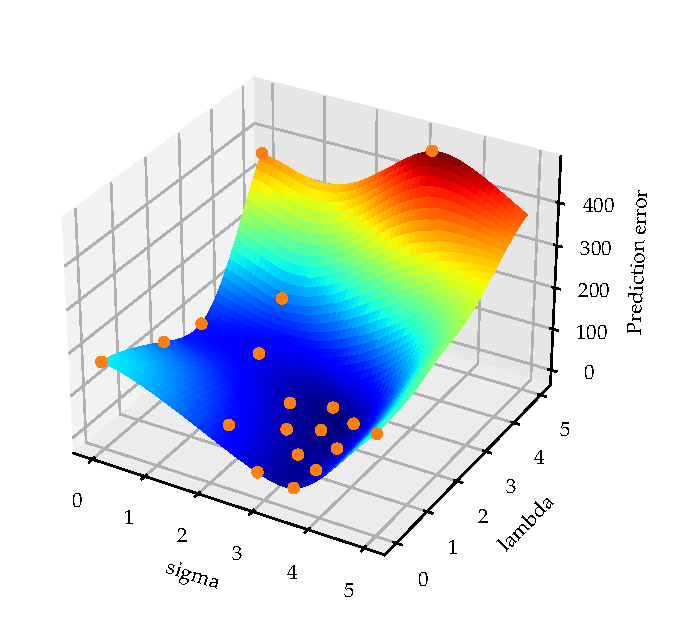
\includegraphics[width=0.46\textwidth]{Pictures/BO_vs_Grid1.eps} }%
    \caption{Example of an optimization task tuning a parameterised regression model with parameters
    $\lambda$ and $\sigma$, on a test set, i.e. minimization of prediction error. We see the first
    23 evaluations out of 100 in grid search vs 23 evaluations using a sample-efficient solver (Bayesian
    optimization). This illustrates the idea of a sample-efficient solver}%
    \label{fig:example}%
\end{figure}

\subsection{Exploitation and exploration}
The balance between an optimization procedure's local/exploitation and global/exploration elements
is key to its performance (statement in thesis \cite{PhDthesis} ok?). Explained here:
\begin{enumerate}
    \item Local element: Exploiting the obtained information $\mathcal{D}$ to find the best point
    \item Global element: Obtaining new information about the characteristics of the objective
    function.
\end{enumerate}
Essentially, the only explorative phase of the deterministic surrogate optimization is the first
initial samples from the objective, i.e. when creating the initial $\mathcal{D}$. If done poorly,
the optimization might get stuck in a local minimum. This is a consequence of their nonexisting
ability to express uncertainty about the objective function. Deterministic surrogate models do not
pay attention to less-explored regions, which is the essential characteristic of a global
optimization method \cite{GlobalOptimization}. 

Bayesian formalism is a powerful and sound tool for incorporating uncertainty into the surrogate
model. Prior to any observed data, we can easily integrate our beliefs about the distribution of
the objective function. When observing data, the likelihood and prior collaborate to create a
predictive (posterior) distribution, $p(y|x,\mathcal{D})$. The next location $x$ to explore is now
determined with a theoretically motivated policy (acquisition function) which might balance the
exploitation and exploration tradeoff. 

Moreover, Bayesian optimization (or \textit{probabilistic} surrogate-based optimization) is motivated by
its ability to deal with noisy objective functions. 


\subsection{Noisy objective functions}
Many optimization algorithms assume \textit{exact} evaluations of the objective function. However,
this assumption is often wrong, especially for objective functions with real-life experiments,
imperfect simulations, human interaction where measurement noise is well known. A potentially noisy
objective function is the main reason why we in Algorithm \eqref{algOPT} use the terminology
$\text{observe}(x)$ and not just \textit{evaluate }$f(x)$.

The observation model is typically noisy and described as
$$y = f(x)+\epsilon$$ where $\epsilon$ is the measurement error, this is
typically assumed to be Gaussian with zero mean and a variance
$\sigma^2$ (which could depend on $x$ in a heteroskedastic setting) and implies a Gaussian observation model, 
$$p(y|f(x),\sigma^2) = \mathcal{N}(y|f(x),\sigma^2)$$ 

% (note from now on we define $\phi := f(x)$ in order to avoid confusion and a extra set of paranteses)
% $$p(y|x,\phi,\sigma) = \mathcal{N}(y;\phi,\sigma^2)$$ 
\begin{note2}["Sampling" from objective function]
    The terminology \textit{to sample} is refering to a probabilistic observation model. Formally, we
    can extend this model to deal with noiseless observations as well, simply by setting
    $\sigma = 0$ and letting the model colaps into a Direct delta distribution, $p(y|f(x)) =
    \mathcal{\delta}(y-f(x))$, i.e. all probability mass for $y$ is on the value $f(x)$ giving the
    observation sample $y = f(x)$. 
\end{note2}

% \begin{note}
%     \textbf{"Sampling" from objective function} 
%     The terminology \textit{to sample} is refering to a probabilistic observation model. Formally, we
%     can extend this model to deal with noiseless observations as well, simply by setting
%     $\sigma = 0$ and letting the model colaps into a Direct delta distribution, $p(y|f(x)) =
%     \mathcal{\delta}(y-f(x))$, i.e. all probability mass for $y$ is on the value $f(x)$ giving the
%     observation sample $y = f(x)$. 
% \end{note}

Bayesian optimization or probabilistic surrogate-based optimization deals with both noiseless and noisy objective functions,
as it defines a Bayesian regression model over the observations.

% \begin{figure}[h]
%     \centering
%     \includegraphics[width=0.9\textwidth]{Pictures/BO_vs_Grid2.eps}
%     \caption{Hyper parameter tuning of a model $M(\lambda, \sigma)$, 
%     35 evaluation in grid search vs 39 evaluations using Bayesian optimization}
%     \label{optimhist}
% \end{figure}

\begin{testexample}[Bayesian Optimization]
    Bayesian optimization is a \textit{probabilistic} surrogate-based optimization
    methodology. Here a cheap probabilistic regression model $p(y|x)$ is fitted to the
    the observations $\mathcal{D}$ and in contrast to (deterministic) surrogate-based
    optimization, it is not possible right away to find the minima in the cheap
    surrogate model; first, we need to interpret the meaning of minima in a probabilistic
    regression model. This interpretation is done through a so-called acquisition
    function (more about this later). The policy is as following,
    $$\text{policy}_{BO}(\mathcal{D}) = \max_x AQ(p(y|x,\mathcal{D}))$$

    \begin{figure}[H]
        \begin{minipage}[c]{0.67\textwidth}
          \includegraphics[width=\textwidth]{Pictures/BO_example.pdf}
        \end{minipage}\hfill
        \begin{minipage}[c]{0.3\textwidth}
          \caption{Top: Bayesian regression model (Gaussian Process) is fitted to the observed data,
          which are sampled from the underlying objective (black sin-function). Bottom: The expected improvement
          \textit{acquisition function} is maximied at the orange arrow, i.e. the location of the
          next sample.  $\text{policy}_{BO}(\mathcal{D}) = 26,06$} \label{BO_example}
        \end{minipage}
    \end{figure}
\end{testexample}


% \begin{tcolorbox}[
%     sharp corners,
%     boxrule=0mm,
%     enhanced,
%     borderline west={4pt}{-2pt}{darkred},
%     borderline north={1pt}{0pt}{darkred},
%     borderline south={1pt}{0pt}{darkred},
%     borderline east={1pt}{0pt}{darkred},
%     %colframe=darkred!0,
%     %colback=darkred!10,
%     %coltitle=darkred,
%     %boxsep=3pt,left=4pt,right=4pt,top=2pt,bottom=2pt
% ]
% { \textcolor{darkred}{\textbf{Example: Bayesian Optimization}}}\\
%     Bayesian optimization is a \textit{probabilistic} surrogate-based optimization
%     methodology. Here a cheap probabilistic regression model $p(y|x)$ is fitted to the
%     the observations $\mathcal{D}$ and in contrast to (deterministic) surrogate-based
%     optimization, it is not possible right away to find the minima in the cheap
%     surrogate model; first, we need to interpret the meaning of minima in a probabilistic
%     regression model. This interpretation is done through a so-called acquisition
%     function (more about this later). The policy is as following,
%     $$\text{policy}_{BO}(\mathcal{D}) = \max_x AQ(p(y|x,\mathcal{D}))$$

%     \begin{figure}[H]
%         \begin{minipage}[c]{0.67\textwidth}
%           \includegraphics[width=\textwidth]{Pictures/Test1Gaussian_Process_-_sklearn000.pdf}
%         \end{minipage}\hfill
%         \begin{minipage}[c]{0.3\textwidth}
%           \caption{Top: Bayesian regression model (Gaussian Process) is fitted to the observed data,
%           which are sampled from the underlying black objective. Bottom: The expected improvement
%           \textit{acquisition function} is maximied at the orange arrow, i.e. the location of the
%           next sample.  $\text{policy}_{BO}(\mathcal{D}) = -79,27$} \label{fig:03-03}
%         \end{minipage}
%     \end{figure}
   
% \end{tcolorbox}


% \begin{algorithm}[H]
%     \caption{Bayesian Optimization}
%     \begin{algorithmic}
%     \State \textbf{Input:} Initial dataset $\mathcal{D}$, Bayesian regression model.
%     \While{Temination is not reached}
%         \State Fit Bayesian regression model: $$p(y|x,\mathcal{D}) = \int p(y|x,\theta)p(\theta|\mathcal{D})d\theta$$
%         \State $x \gets \max_x AQ(p(y|x,\mathcal{D}))$\Comment{Find point with highest acquisition}
%         \State $y \gets \text{observe}(x)$ \Comment{observe objective function at chosen location}
%         \State $\mathcal{D} \gets \mathcal{D} \cup \{(x,y)\} $ \Comment{update dataset}
%     \EndWhile
%     \State $\textbf{return: } \mathcal{D}$
%     \end{algorithmic}
% \end{algorithm}


% \begin{mybox}{darkred}{A red box}
%     Test
% \end{mybox}

% <Cope with inacuracies> i.e. allows for stochastic objective function. 
% <Uncertainty measure with prediction based on simple and clear prior 
% assumptions about the characteristic about the objective function. >
% <Provides an adequate termination condition for the opt. process>. 

% <kilde 151. Bayes Opt is assumed superior to other global optimization technics 
% with limited budget>

\section{Bayesian regression}
% \begin{testexample2}[Bayesian methodology]
%     In Bayesian statistics $p(\theta|\mathcal{D})$ is the posterior distribution, and it is 
% of $\theta$ is linked to the likelihood and prior via Bayes rule,
% $$p(\theta|\mathcal{D}) = \frac{p(\mathcal{D}|\theta)p(\theta)}{p(\mathcal{D})}$$
% \end{testexample2}
Whereas traditional regression workflow is the following: Given data, choose the best fitting model
parameters, make predictions using those parameters. The Bayesian framework allows us to skip the
dependency of a single set of parameters and instead use \textit{all possible} parameters by treating the set
of parameters as a random quantity, $\theta \sim p(\theta|\mathcal{D})$, where some values/realizations of $\theta$ are more
probable than others given data. In Bayesian regression we are interest is the predictive posterior distribution,  
\begin{align}\label{Predictive2}
    p(y|x, \mathcal{D}) &= \int p(y,\theta|x, \mathcal{D}) d\theta\\
    &= \int p(y|x,\theta)p(\theta|\mathcal{D}) d\theta,
\end{align}
where the posterior $p(\theta|\mathcal{D})$ gives weighting to the proposed regression model
$p(y|x,\theta)$. Note that the second equation is true because of the probability chain rule and
that $y$ is fully described by the parametric model $p(y|x,\theta)$ and the parameters $\theta$ are
fully described by the posterior distribution $p(\theta|\mathcal{D})$.


\subsection{Surrogate model}
A surrogate model in a Bayesian optimization setting is a Bayesian regression model. The most
used surrogate model is a Gaussian Process. But there have been investigations on other 
surrogates, such as Bayesian neural networks and Bayesian regression trees. These are all
discriminative models, and another approach we focus on in this project is to model $y$ and
$x$ jointly in a so-called generative model, $p(x,y)$. A generative model can be used implicitly
as a surrogate from the conditional distribution of $y$ given $x$, $p(y|x)$.

In this thesis, the Bayesian regression models investigated as Bayesian optimization surrogates are
the following:
\begin{itemize}[noitemsep]
    \item Gaussian process (GP)
    \item Bayesian neural network (BNN)
    \item Kernel density regression (KDE)
    \item Gaussian mixture regression (GMR)
    \item Sum-product networks (SPN)
\end{itemize}

We now introduce the concept of inference, which is necessary for using the probabilistic surrogate models
in Bayesian Optimization. 

\subsection{Inference of surrogate models}
Inference is the process of computing answers to queries about a probabilistic model after observing
data. In Bayesian regression, the query is the predictive distribution, $p(y|x,\mathcal{D})$, as we
are interested in the distribution of $y$ given $x$ and already observed data, $\mathcal{D}$. This
often indirectly create the posterior query, $p(\theta|\mathcal{D})$, the probability of model
parameters $\theta$ given data $\mathcal{D}$. Lastly, it is also inference when we train a Gaussian
mixture model or SPN using the expectation-maximization algorithm (EM) since we are iteratively
answering the query $E_{p(z|\theta^{(k)})}[z|\theta]$.

%\subsection{Exact and approximate inference}
We distinguish between two different ways of inference: Exact and approximate inference. It is
\textit{exact inference} when a probabilistic query is calculated exact. It is possible to
calculate exact inference on the predictive distribution for the Gaussian mixture model, Sum product
network, and Gaussian processes. Models which allow for exact inference have a powerful advantage
over the models with approximate inference since we can guarantee the answers to the queries are
correct; however, they are usually also less expressive (unable to explain complicated models). 

When it is not possible to answer a probabilistic query exact, we can approximate the answer using
\textit{approximate inference}. When dealing with complicated and expressive statistical models,
exact inference is often intractable, and we need to use approximate inference. Approximate
inference is a broad category of methods, which includes variational inference and Markov chain
Monte Carlo (MCMC). The two Bayesian Neural networks, we deal with in this project, Bohamiann and
Numpyro BNN are similar regression models but are inferred using two different MCMC methods,
Hamiltonian Monte Carlo - giving different results. As revealed later (see in section \ref{BNN})
approximate inference might be flawed and inexact. 

\begin{table}[H]
    \centering
    \begin{tabular}{l|l|l}
    %\rowcolor[HTML]{C0C0C0} 
    \textbf{Model}       & \textbf{Predictive inference}    &   \textbf{Learning} \\ \hline
    GP                          & Exact $O(n^3)$            & Emperical Bayes\\
    Numpyro BNN                 & No U-Turn Sampler         & \\
    Bohamiann BNN               & Adaptive stochatic HMC    & \\
    Kernel density regression   & Exact $O(n)$              & \\
    Gaussian mixture regression & Exact $O(K)$              & EM  \\
    SPN                         & Exact $O(E)$              &  EM $O(E)$\\
    \end{tabular}
    \caption{Overview of inference methods applied on the statistical models used in this project.
            $E$ is the number of edges in the SPN. $n$ is the number of data points. $K \leq n$ is
            the number of mixture components. We will soon learn that for an SPN the number of
            mixture components is exponentially larger than the number of edges i.e. $E << K$. In theory
            MCMC methods samples from true the posterior distribution, and do not need any
            fitting/learning. }
\end{table}

\newpage
\section{Acquisition function}
Given a correct predictive distribution $p(y|x\mathcal{D})$ the next step in Bayesian optimization
is to select the next location $x \in \mathcal{X}$ to sample from. The next location is chosen
according to a so-called acquisition function (AQ function), which balances out the well-known
concept of exploitation and exploration. It is exploitation if the next chosen location according to
its average improvement. It is exploration if the next point is chosen in a region of high
uncertainty and thereby helps lower the overall uncertainty. First, we will look at the acquisition
function used in the thesis: Expected improvement. Secondly, we shortly present other different
types of acquisition functions. In Figure \ref{Different_AQ_functions} we see three different
acquisition functions. The expected improvement (EI) is known for being biased towards exploitation.
In contrast, the negative lower confidence bound (LCB) has a parameter $\beta$, which can be tuned
to make it focus more on exploration. 
\begin{figure}[H]
    \centering
    \includegraphics[trim=1cm 0cm 1cm 1cm,clip,width=\textwidth]{Pictures/illustration_AQs.pdf}
    \caption{The same regression model and points as Figure \ref{BO_example}, but with three
    different acquisition functions: Expected improvement and negative lower confidence bound for
    two different lower quantiles $0.841$ and $0.999$. The latter yields more exploration.}\label{Different_AQ_functions}
\end{figure}

\begin{figure}[H]
    \centering
    \begin{minipage}[b]{0.32\textwidth}
      \includegraphics[trim=0.2cm 0.2cm 0cm 0.1cm,clip,width=\textwidth]{Pictures/expected_improvement_illustration.pdf}
    \end{minipage}
    \hfill
    \begin{minipage}[b]{0.32\textwidth}
        \includegraphics[trim=0.2cm 0.2cm 0cm 0.1cm,clip,width=\textwidth]{Pictures/neg_lower_confidence_illustration_1.pdf}
      \end{minipage}
     \hfill
     \begin{minipage}[b]{0.32\textwidth}
        \includegraphics[trim=0.2cm 0.2cm 0cm 0.1cm,clip,width=\textwidth]{Pictures/neg_lower_confidence_illustration_3.pdf}
      \end{minipage}
    \caption{Contourplot of expected improvement and lower confidence bound (for two different
    quantiles) for different (Gaussian) predictive uncertainties $\sigma_x =
    \sqrt{\mathbb{V}ar_{p(y|x,\mathcal{D})y]}}$ versus the average improvement $y_{\min}-\mu_x$,
    where $\mu_x = E_{p(y|x,\mathcal{D})}[y]$ (high values are dark). The colored lines are the
    mapping $x \mapsto (\sigma_x, y_{\min}-\mu_x)$ for $x = [-100, 100]$ for the Bayesian regression
    function in Figure \ref{Different_AQ_functions} - and thereby explains how the acquisition
    functions balances exploitation and exploration. The orange dot represent the point maximizing
    the acquisition function}
    \label{EI_illustration}
\end{figure}


\subsection{Expected improvement}
A popular choice of acquisition function is expected improvement, 
$$EI(x) = \mathbb{E}_{p(y|x,\mathcal{D})}[\max(0, y_{\min}-y)]$$ where we only consider the values
$y$, which improves the current best value in the expectation of the predictive distribution,
$p(y|x,\mathcal{D})$. Therefore, a $x$ which yield a bad predictive mean value
$\mathbb{E}_{p(y|x,\mathcal{D})}[y]> y_{\min}$ might still be maximizing the expectated improvement,
if the predictive uncertainty is very large at $x$. Figure \ref{EI_illustration} illustrates that a
large uncertainty in the predictive distribution (represented as the predictive variance) can lead
to relative large values even for non-improving mean predictions.


\begin{note2}[Why defining expected improvment with max]    
    Note that $\max(0,\cdot)$ is important since the Bayesian optimization othervise reduces to
    a simple non-probabilistic surrogate-based optimization method,
    \begin{align*}
        \mathbb{E}_{p(y|x,\mathcal{D})}[y_{\min}-y] = y_{\min} - \mathbb{E}_{p(y|x,\mathcal{D})}[y]
    \end{align*}
    i.e. maximizing the above is equivalent to maximizing the predictive mean, and thereby we loose
    all the valuable information about the predictive uncertainties from the Bayesian regression model. 
\end{note2}

\subsubsection{Exact expected improvement} \label{ExactEI} 
In the following derivation we assume the
predictive distribution can be approxiamted by a normal distribution dependent on the point of
interest $x$ and the data $\mathcal{D}$ (note for the GP it is in fact not an approximation), 
$$p(y|x,\mathcal{D}) \approx \mathcal{N}(y|\mu(x,\mathcal{D}), \sigma^2(x,\mathcal{D}))$$ where we
will change to a less clumpsy notation $\mathcal{N}(y|\mu_x,
\sigma^2_x):=\mathcal{N}(y|\mu(x,\mathcal{D}), \sigma^2(x,\mathcal{D}))$. This is completely fine
since we $x$ is fixed (and $\mathcal{D}$ is fixed) when evaluating the expected improvement in a point
$x$. %  $\sigma_x := \sigma^2(x,\mathcal{D})$ and $\mu_x := \mu(x,\mathcal{D})$
%as evaluated functions, i.e. numbers. 
Furthermore, the density of
a standard normal distribution is denoted $\phi(\cdot):=\mathcal{N}(\cdot | 0,1)$, and the cumlative
density function (CDF) of a standard normal distribution is denoted, $\Phi(\cdot) :=
\int_{-\infty}^{\cdot} \phi(\epsilon)d\epsilon$. We will now see that the normal approximation
of the predictive distribution yiels closed form solution to the expected improvement function, 

\begin{align*}
    E_{\mathcal{N}(y|\mu_x, \sigma_x^2)}[\max(0,y_{\min}-y)] &= \int \max(0,y_{\min}-y) \mathcal{N}(y|\mu_x, \sigma_x^2) dy\\
    &= \int_{-\infty}^{y_{\min}} (y_{\min}-y) \frac{1}{\sigma_x}\phi\left(\frac{y-\mu_x}{\sigma_x}\right) dy\\
    &= \int_{-\infty}^{\frac{y_{\min}-\mu_x}{\sigma_x}} (y_{\min}-\mu_x-\sigma_x\epsilon) \frac{1}{\sigma_x}\phi\left(\epsilon\right) \sigma_x d\epsilon\\
    &= \int_{-\infty}^u \sigma_x \cdot (u-\epsilon) \phi(\epsilon) d\epsilon\\
    &=  \sigma_x \cdot \left( u\cdot \int_{-\infty}^u \phi(\epsilon) d\epsilon +\int_{-\infty}^u (-\epsilon)  \phi(\epsilon) d\epsilon \right) \\
    &= \sigma_x [u\Phi(u)+ \phi(u)]
\end{align*}

where $u:=\frac{y_{\min}-\mu_x}{\sigma_x}$. 

\begin{note2}[Derivation details]
    To understand the identity $\phi(u) = \int_{-\infty}^u
    (-\epsilon)  \phi(\epsilon) d\epsilon$ used in the last equality, we first see that the antiderivative
is $\phi(\epsilon) = \frac{1}{\sqrt{2\pi}} \exp\left(\frac{-\epsilon^2}{2}\right)$,
\begin{align*}
    \frac{d}{d \epsilon} \phi(\epsilon) =  \frac{1}{\sqrt{2\pi}}\frac{d}{d \epsilon}  \exp\left(\frac{-\epsilon^2}{2}\right) 
    =  \frac{1}{\sqrt{2\pi}}\exp\left(\frac{-\epsilon^2}{2}\right)(-\epsilon)
    = -\epsilon \phi(\epsilon)
\end{align*}
and evaluating the rieman integral is equivalent to evaluate the antiderivative in its boundaries, giving the 
solution, 
$$\int_{-\infty}^u
(-\epsilon)  \phi(\epsilon) d\epsilon = \left[\phi(\epsilon)\right]_{-\infty}^u = \phi(u)-0 = \phi(u)$$ 
\end{note2}

We can also explicily write the expected improvement as, 
$$EI(x) = (y_{\min}-\mu_x)\Phi\left(\frac{y_{\min}-\mu_x}{\sigma_x}\right)+ \sigma_x
\phi\left(\frac{y_{\min}-\mu_x}{\sigma_x}\right)$$ where the first part can be interpretted as
exploitation (favouring points with a large average improvement $I(x) := (y_{\min}-\mu_x)$) and the second
part can be seen a exploitation (favouring points with high uncertainty.). This can also be seen
in Figure \eqref{EI_illustration}, where it is clear that the expected improvement is growing for
growing average improvement $I(x)$ and also for growing prediction uncertainty $\sigma_x$.


% taking the derivative with
% respect to $I(x) := (y_{\min}-\mu_x)$ and $\sigma_x$, we see that expected improvement is is
% increasing if the improvement grows or if the variance $\sigma_x$ grows, i.e
% $$\frac{\partial EI(x)}{\partial I(x)} = \Phi\left(\frac{y_{\min}-\mu_x}{\sigma_x}\right) > 0, \hspace*{0.5cm} 
% \frac{\partial EI(x)}{\partial \sigma_x} = \phi\left(\frac{y_{\min}-\mu_x}{\sigma_x}\right) >0$$ 
% <obs mistake in the book!!!?>

\subsubsection{Approximate expected improvement}
If the predictive distribution is non-Gaussian, it is either possible to approximate it as a Gaussian
(By using the mean and variance of the predictive distribution to define the Gaussian approximation)
or calculate the expected improvement approximately as follows, 
\begin{align*}
    E_{p(y|x,\mathcal{D})}[\max(0,y_{\min}-y)] &= \int \max(0,y_{\min}-y) p(y|x,\mathcal{D}) dy\\
    &\approx \frac{1}{K} \sum_{k=1}^K  \max(0,y_{\min}-y^{(k)})
\end{align*}
where $y^{(k)}$ are samples from the predictive distribution.

% In the case of a parametric model
% like a Bayesian NN, then we already got posterior samples from posterior $\theta^{(k)} \sim p(\theta | \mathcal{D})$, giving, 
% $$p(y|x,\mathcal{D}) \approx \frac{1}{K_2} \sum_{k=1}^{K_2} p(y|x,\theta^{(k)})$$ where
% $p(y|x,\mathcal{D} = \mathcal{N}(y|NN_w,\sigma))$. So essentially we should sample from a sampled
% distribution, but instead the PhD thesis \cite{PhDthesis}, just sample the mean and set $K_2 = 1$... 


% \begin{align*}
%     \mathbb{E}_{y_*|\textbf{x}_*,D_n}[\max(0,y_{\min}-y_*)] &= ??\\
%     \mathbb{E}[\min(0,y_{\min}-y_*)|\textbf{x}_*,D_n] &= \int_{-\infty}^\infty \min(0,y_{\min}-y_*) p(y_*|\textbf{x}_*,D_n) dy_*\\
%     &= \int_{-\infty}^{y_{\min}} (y_{\min}-y_*) p(y_*|\textbf{x}_*,D_n) dy_*\\
%     &\approx \frac{1}{N} \sum_{\theta \in \Omega } [y_{\min}-f_\theta(x)]
% \end{align*}

% where $\Omega = \{\theta|f_{\theta}(x)< y_{\min}\}$

%\section{uncertainties}
%Alatoric vs epistemic uncertainties 

\subsection{Lower confidense bound}
Lower confidence bound is defined by a confidence paramter $\pi \in [0,1]$
and then the lower quantile $\int_{\infty}^x p(y|x,\mathcal{D})dy = (1-\pi)$
is chosen as the acquisition. For a Gaussian predictive distribution this is 
simply  <more..>
$$nLCB(x) = - (\mu_x - \beta \sigma_x)$$
where $\beta = \Phi^{-1}(1-\pi)$.  
% \begin{figure}[H]
%     \centering
%     \includegraphics[width=\textwidth]{Pictures/neg_lower_confidence_illustration.pdf}
%     \caption{<Soon similar plot as Figure \ref{EI_illustration}> Illustration of the values of the
%     negative lower confidence bound for different predictive uncertainties $\sigma_x =
%     \sqrt{\mathbb{V}ar_{p(y|x,\mathcal{D})}[y]}$ versus the average improvement $y_{\min}-\mu_x$,
%     where $\mu_x = E_{p(y|x,\mathcal{D})}[y]$}
%     \label{nLCB_illustration}
% \end{figure}

\subsection{Entropy search}

<copy> An information theoretic approach
which accounts for the overall information gain on the optimizer ob-
tained from a new evaluation has also been presented. This is known
as informational approach to global optimization (IAGO), and uses en-
tropy as a measure for information (Villemonteix, Vazquez, and Walter,
2009).

\subsection{probability of improvement}


% We then discuss the knowledge
% gradient (Section 4.2), entropy search, and predictive entropy search (Section 4.3) acquisition functions.
% These alternate acquisition functions are most useful in exotic problems where an assumption made by
% expected improvement that the primary benefit of sampling occurs through an improvement at the point
% sampled is no longer true.


% The entropy search (ES) (Hennig and Schuler, 2012) acquisition function values the information we have
% about the location of the global maximum according to its differential entropy

% ES seeks the point to evaluate what causes the largest decrease in differential entropy

% (Recall from, e.g., Cover and Thomas (2012),
% that the differential entropy of a continuous probability distribution p(x) is R
% p(x) log(p(x)) dx, and that
% smaller differential entropy indicates less uncertainty.)

% Predictive entropy search (PES) (Hern´andezLobato et al., 2014) seeks the same point but uses a reformulation of the entropy reduction objective
% based on mutual information. Exact calculations of PES and ES would give equivalent acquisition functions, but exact calculation is not typically possible, and so the difference in computational techniques
% used to approximate the PES and ES acquisition functions creates practical differences in the sampling
% decisions that result from the two approaches. We first discuss ES and then PES.

% Let x  be the global optimum of f. The posterior distribution on f at time n induces a probability
% distribution for x
% . Indeed, if domain A were finite, we could represent f over its domain by a
% vector (f(x): x ∈ A), and x
% would correspond to the largest element in this vector. The distribution of
% this vector under the time-n posterior distribution would be multivariate normal, and this multivariate
% normal distribution would imply the distribution of x

% . When A is continuous, the same ideas apply,
% where x

% is a random variable whose distribution is implied by the Gaussian process posterior on f




% With kriging, we can develop search methods that put some emphasis on sampling where the standard
% error is high. In this way, we obtain the desired feature of ‘paying attention to parts of the space
% that have been relatively unexplored.’
\cleardoublepage

\chapter{Bayesian regression models - probabilistic surrogate model}
As mentioned in the previous sections, the first of two repeated steps in Bayesian optimization
is to create a good Bayesian regression model. %why not non bayesian regression? 
i.e. finding the probility of prediction for a arbitrary point $x$ given datapoints 
$\mathcal{D} = \{x_1, y_1, \dots, x_n, y_n\}$, 
 $$p(y|x,\mathcal{D})$$

The surrogate model of choise in Bayesian optimization is a Gaussian Process, and Bayesian Neural Network.
These are discriminative models, however, another approach, which we focus on in this project, is
to model $y$ and $x$ jointly in a so-called generative model.

\section{Gaussian mixture regression}
Taking a convex combination of a set of multivariate Gaussian distributions is a Gaussian mixture model
$$p(z) = \sum_{k=1}^K \pi_k \mathcal{N}(z|\mu_k, \Sigma_k)$$  
Defining $z := (x,y)$ we can model our data, as a generative model $p(x,y)$, now, since the conditonal 
of a Gaussain mixture again is Gaussain mixture - i.e. closed form expression, we can exactly calculate
$p(y|x) = GMM_{y|x}$

Assuming iid data the likelihood is given as 
$$p(\mathcal{D}|\mu_1, \dots, \mu_K, \Sigma_1, \dots, \Sigma_K, \pi_1, \dots, \pi_K) = \prod_{i=1}^n \sum_{k=1}^K \pi_k \mathcal{N}(z_i|\mu_k, \Sigma_k)$$
And the log likelihood, 
$$\log p(\mathcal{D}| ..) = \sum_{i=1}^n \log \sum_{k=1}^K \pi_k \mathcal{N}(z_i|\mu_k, \Sigma_k)$$


\section{Mixture regression in a Bayesian setting}
As seen in examples. The uncertainty of conditional distribution is way too certain
in areas with no data points, therefore we need to enhance the model with some bayesian 
flavour. 

$$p(y|x,\mathcal{D}) = p(y|x,Z)p(Z|x)$$



\subsection*{Expetation-maximization algorithm}
A way to find local maxima in the likehood function is using the EM algorithm. 

If we define a latent/hiddem random variabel $Z_i \in \{1,\dots, K\}$ for each data point, then 
the likelihood function becomes, 
$$L(\theta|\mathcal{D}, Z) = \prod_{i=1}^n \sum_{k=1}^K 1(Z_i = k) \pi_k \mathcal{N}(z_i|\mu_k, \Sigma_k)$$

Now the expectation wrt. the current value $p(Z|\mathcal{D}, \theta^k)$ is given as 
$$Q(\theta|\theta^k) = \mathcal{E}_{p(Z|\mathcal{D}, \theta^k)}=L(\theta|\mathcal{D}, Z) $$

And then update the next parameter estimate with
$$\theta^{k+1} = \arg \max_{\theta} Q(\theta|\theta^k)$$

This is repeated untill convergence. 


\section{Sum product networks}
We will for a large extend just see SPN as a large mixture model. This is a totally valid observation. 

\subsection*{Mixture model}
%from [@desana]:
\begin{definition} 
    A sub-network $\bar S_z$ of $S$ is an SPN, which includes the root $S$ and then includes nodes
    according to the following recursive scheme: 
\end{definition}
\begin{algorithm}[H]
    \caption*{Collection of sub-network $S_z$ of $S$}\label{SPN3}
    \begin{algorithmic}
    %\State \textbf{Global:}  $S_z$ 
    \Function{Process}{node i, $S_z$}
    \If{$i \in \mathcal{L}eaf(S)$}
        \State  $\textbf{return: }$ 
    \EndIf
    %\For{$i \in I_{o}$}
    \If{$i\in \mathcal{S}um(S)$}
       %\State $S_z =S_z \cup \{j \in ch(i)\}$ \Comment{include one child of node $i$}
        \State $S_z =S_z.add(j \in ch(i))$ \Comment{include one child of node $i$}
        \State $\textbf{return: } \text{Process}(j, S_z)$
    \EndIf
    \If{$i\in \mathcal{P}rod(S)$}
        \State $S_z =S_z \cup \{j | j \in ch(i)\}$ \Comment{include all childen of node $i$}
        \For{$j \in ch(i)$}
            \State $\textbf{return: } \text{Process}(j,S_z)$
        \EndFor
    \EndIf
    \State $\textbf{return: } S_z$
    \EndFunction
    \State $S_z =  \text{Process(root,Ø)}$
    \end{algorithmic}
\end{algorithm}
So we see that at each sum node the number of different sub-networks multiplies with the number of children for that
sum node. And thereby, the total number of sub-networks is
 $$Z = \prod_{i\in \mathcal{S}um(S)}|ch(i)|$$ 
 i.e. an exponential large amount of sub-networks. This is the amount of
 mixture components implicitly defined in an SPN. 
 Denote the set of edges in the sub-network $\mathcal{E}(S_z)$.
Now the we define a mixture coeficient, $\lambda_z$ and component for each $S_z$ as 
$$\lambda_z := \prod_{(i,j)\in \mathcal{E}(S_z)} w_{i,j}, \hspace{1cm}
p_z(x,y|\theta) := \prod_{i \in \mathcal{L}(S_z)} p_i(x,y)$$
where $p_i(x,y)$ is the leaf distribution at leaf node $i$ paramitised with $\theta$. 
It can now be proven that the SPN can be interpreted as the following mixture model, 
$$p(x,y|w,\theta) = \sum_{z=1}^Z \lambda_z(w)p_z(x,y|\theta)$$
i.e. by the weighted sum of all $Z$ sub-networks. For convinience
we define each sum component as $p(z,x,y|w,\theta) := \lambda_z(w)p_z(x,y|\theta)$.
Evaluation of $p(x,y|w,\theta)$ will never be done as the sum over $Z$ components, 
instead there is a proposition. 

\begin{proposition}
    Consider a SPN, S, a sum node $q \in \mathcal{S}um(S)$ and a child $i \in ch(q)$,
    then the following relation holds, 
    $$\sum_{z:(q,i)\in \mathcal{E}(S_z)} \lambda_z(w) p_z(x,y|\theta) = w_{i,q}
    \frac{\partial S}{\partial v(q)} v(i)$$
\end{proposition}



\subsection*{Conditional of SPN}

We will soon see how it is possible to write the conditional distribution as the mixture, 
$$p(y|x) = \sum_{z \in \Sigma(S)} \gamma(x) p_{z_y}(y)$$
where $ \Sigma(S)$ is the set of all sub-networks in the SPN, $S$ - \todo{IT IS EXPONENTIALLY LARGE}.  
And where $p_{z_y}(y)$ is defined through $p_z(x,y)$, 
\begin{align*}
    p_z(x,y) &= \prod_{l \in \mathcal{L}eaf(z_x)} \phi_l(x)\prod_{l \in \mathcal{L}eaf(z_y)} \phi_l(y)\\
            &=: p_{z_x}(x) p_{z_y}(y) 
\end{align*}
where $\phi_l$ is the density of the $l$'th leafs tractable distribution. Recall that we can interpret an SPN
as the mixture model, 
$$p(x,y) = \sum_{z \in \Sigma(S)} \lambda_z p_z(x,y)$$
where $\lambda_z = \prod_{(q,j) \in \mathcal{E}(z)} w_{q,j}$. First we calculate the marginal density,
$p(x)$, 
\begin{align*}
    p(x) &= \int p(x,y)dy\\
    &= \int \sum_{z \in \Sigma(S)} \lambda_z p_z(x,y)dy\\
    %&= \sum_{z \in \Sigma(S)} \lambda_z  \int p_z(x,y)dy\\
    &= \sum_{z \in \Sigma(S)} \lambda_z p_{z_x}(x)\int p_{z_y}(y)dy \\
    &= \sum_{z \in \Sigma(S)} \lambda_z p_{z_x}(x)
\end{align*}
Now we are ready to calculate the conditional density, 
\begin{align*}
    p(y|x) &=  \frac{p(x,y)}{p(x)}\\
            &= \frac{\sum_{z \in \Sigma(S)} \lambda_z p_z(x,y)}{p(x)}\\
            &=\sum_{z \in \Sigma(S)}\frac{ \lambda_z p_{z_x}(x)}{p(x)} p_{z_y}(y)\\
            &=\sum_{z \in \Sigma(S)}\frac{ \lambda_z p_{z_x}(x)}{\sum_{z \in \Sigma(S)} \lambda_z p_{z_x}(x)} p_{z_y}(y)\\
            &=\sum_{z \in \Sigma(S)} \gamma(x) p_{z_y}(y)
\end{align*}
So we defined $\gamma(x) = \frac{ \lambda_z p_{z_x}(x)}{\sum_{z \in \Sigma(S)} \lambda_z p_{z_x}(x)}$ 
and this is very convinient, as we will see soon is 
equavalent to the derivative of the log-likehood
of the SPN, which is easily obtained by automatic differentiation. 

\subsection*{calculation of $\gamma(x)$}
expectation maximization of a mixture model, is given by Bishop..
the responsibility of a datapoint to belong to one mixture component, is given by
$$\gamma(z_{nk}) = \frac{w_k p_j(x_n)}{\sum_i w_i p_i(x_n)}$$
We can prove that the responsibility is equal to the gradient of the log likehood, 
$$L:= \sum_n \log \sum_j w_j \exp \psi_j(x_n)$$
where we define $\psi_j(x_n) = \log p_j(x_n)$. Take the gradient 
$$\frac{\partial L}{\partial \psi_{j}(x_{n})} = \frac{w_k p_j(x_n)}{\sum_i w_i p_i(x_n)}$$
Note that the gradient easily can be found using autograd. 


\subsection*{Mean and variance of $p(y|x)$}

The mean of the conditional is just
\begin{align*}
    E_{p(y|x)}[y] &= \sum_{z \in \Sigma(S)} \gamma(x) \int  y p_{z_y}(y) dy \\
    &= \sum_{z \in \Sigma(S)} \gamma(x) \prod_{l \in \mathcal{L}eaf(z_y)} E_{\phi_l}[y]
\end{align*}

and the variance is found using the second moment, 
\begin{align*}
    E_{p(y|x)}[y^2] &= \sum_{z \in \Sigma(S)} \gamma(x) \int  y^2 p_{z_y}(y) dy \\
    &= \sum_{z \in \Sigma(S)} \gamma(x) \prod_{l \in \mathcal{L}eaf(z_y)} (Var_{\phi_l}[y]+E_{\phi_l}[y]^2)
\end{align*}



SPN is an exponential large mixture model, with linear inference - unlike GMM. !?
\todo{Write naive bayesian mixture model as a Sum Product Network}

sum nodes play a role of
mixtures over their children distribution, similar to a classic mixture model

Product
nodes on the other hand, are equivalent to factorizations over independent distributions as they are
combining disjoint RVs.

SPNs can also be interpreted as deep feed forward neural network [@vergari]. Here, imagine the
weights of the sum nodes are parameters, leaf distributions are input neurons, root node is output and
all other nodes correspond to hidden neurons



\cleardoublepage

\chapter{Inference: Prediction and learning}
% Inference is the task of receiving conclusions from data and quantify the uncertainties of these. These conclusions
% extend beyond the data. A statistical model is essential for making inference. In Bayesian regression we assign uncertainty 
% to the regression parameters i.e. the weights in the deep neural network, or ?? the function values evaluated at given point in
% Gaussian processes. Sum product networks and and mixture models are not Bayesian regression models, however, their conditional
% distribution should be accombined with a prior. 

%We are dealing with probabilistic models paramitised with $\theta$

Inference is the process of computing answers to queries about a probabilistic model after observing data. 
In Bayesian regression, the
query is the predictive distribution, $p(y|x,\mathcal{D})$, as we are interested in the distribution of $y$ given $x$ 
and already observed data, $\mathcal{D}$. 
This often indirectly create the posterior query, $p(\theta|\mathcal{D})$, the probability of model parameters $\theta$ given data
$\mathcal{D}$. Lastly it is also inference, when we train 
a Gaussian mixture model or SPN using the expectation-maximization algorithm (EM), since we are iteratively answering the query
$E_{p(z|\theta^{(k)})}[z|\theta]$.

% in general a probabilistic model is a joint distribution of hidden variables, $z$, and observed variables, $x$, 
% $$p(z,x)$$

% inference about the unknowns is through the posteriror, 
% $$p(z|x) = \frac{p(z,x)}{p(x)}$$
% For most models, the determinator $p(x)$ is intractable. 
% variational inference turns inference into an optimization problem. 

\section{Exact and approximate inference}
We distinguish between two different ways of inference, exact and approximate inference.
It is \textit{exact inference} when a probabilistic query is calculated exact. It is possible to calculate exact inference on 
the predictive distribution for the Gaussian mixture model, Sum product network, and Gaussian processes. Models which allow 
for exact inference have a powerful advantage over the models with approximate inference since we can guarantee
 the answers to the queries are
correct, however, they are usually also less expressive. It is possible to
make exact inference of SPN, Gaussian Process, and Gaussian Mixture Regression. 
% \begin{itemize}
%     \item SPN
%     \item Gaussian Process
%     \item Gaussian Mixture Regression
% \end{itemize}

When it is not possible to answer a probabilistic query exact, we can approximate the
answer using \textit{approximate inference}. When dealing with complicated and expressive statistical models, exact inference is often
intractable and we need to use approximate inference. Approximate inference 
is a broad category of methods, which includes 
variational inference, Laplace approximation, and Markov chain Monte Carlo (MCMC).
The two Bayesian Neural networks we deal with in this project Bohamiann and Numpyro BNN are
similar regression models, but are infered using two different versions of the MCMC 
method, Hamiltonian Monte Carlo. As it will be revealed later (see result section) 
approximate inference might indeed be flawed and inexact. 
%When dealing with complicated and expressive statistical models, exact inference is often
%intractable and we need to use approximate inference, which might indeed be flawed and 
%inexact. 
% \begin{itemize}
%     \item Bohamiann (Adaptive stochastic MCMC)
%     \item Numpyro Bayesian Neural Network (NUTS)
% \end{itemize}

\begin{table}[H]
    \centering
    \begin{tabular}{l|l|l}
    %\rowcolor[HTML]{C0C0C0} 
    \textbf{Model} & \textbf{Predictive inference} &   \textbf{Learning} \\ \hline
    GP          & Exact $O(n^3)$  & Emperical Bayes\\
    SPN             & Exact $O(E)$ &  EM $O(E)$\\
    Gaussian Mixture Regression & Exact $O(K)$ & EM  \\
    Bohamiann                             & Adaptive stochatic HMC & \\
    Numpyro BNN                           & No U-Turn Sampler & 
    \end{tabular}
    \caption{Overview of inference methods applied on the statistical models 
            used in this project. $E$ is the number of edges in the SPN. $n$ is the number of datapoints. 
            $K \leq n$ is the number of mixture comonents. We will soon learn that for an
            SPN the number of mixture compenets is exponential larger than number of edges
            i.e. $E << K$. In theory MCMC methods samples 
            from true the posterior distribution, and do not need any fitting/learning. 
            }
\end{table}

\section{SPN}
Sum-product networks are generative models, i.e. statistical models of the joint distribution $p(x,y)$. 
We need, however, a disciminative model for regression, i.e. 
a model of the conditional distribution $p(y|x)$. 
SPNs allow for exact inference of the joint distribution 
and any marginalized distribution. These combined queries is sufficient for the
exact predictive posterior. 

\subsection{SPN - prediction}
Prior to the inference of the predictive distribution, we assume that the SPN, S, is trained, i.e.
trained leaf distributions $p_j(\cdot)$ for all leaf nodes, 
$j \in \mathcal{L}eaf(S):=\{j \in \mathcal{V}(S) |pa(j) = \text{Ø}\}$ and
weights $w_{i,j}$ for the connections between every sum nodes
$i \in \mathcal{S}$ and its children, $j \in ch(i)$.  
%The indexes of the nodes, are ordered such that leafs are first, and parents of leafs are next and then the grandparents and so on.

The joint and the marginal distribution are evaluated in the following recursive way
\begin{algorithm}
    \caption*{Calculation of $p(x,y)$}\label{SPN_1}
    \begin{algorithmic}
    \State \textbf{Input:} Fully trained SPN, with leaf distributions $p_i(\cdot)$ for $i\in \mathcal{L}eaf(S)$ and weigts 
    $w_{i,j}$ for $(i,j) \in \{(i,j)|i \in \mathcal{S}um(S), j \in ch(i)\}$ 
    \Function{\text{Eval}}{node i}
    \If{$i \in \mathcal{L}eaf(S)$}
        \State  $\textbf{return: } p_i(x,y)$ \Comment{evaluate leaf distributions at point $(x,y)$}
    \EndIf
    %\For{$i \in I_{o}$}
    \If{$i\in \mathcal{S}um(S)$}
        \State $\textbf{return: } \sum_{j\in ch(i)} w_{i,j} \text{Eval}(j)$
    \EndIf
    \If{$i\in \mathcal{P}rod(S)$}
        \State $\textbf{return: } \prod_{j \in ch(i)} \text{Eval}(j)$
    \EndIf
    \EndFunction
    \State $p(x) =  \text{Eval(root)}$
    \end{algorithmic}
\end{algorithm}


% \begin{algorithm}[H]
%     \caption*{Calculation of $p(x,y)$}\label{jointSPN}
%     \begin{algorithmic}
%     \State \textbf{Input:} Fully trained SPN and point $(x,y)$ %with leaf distributions $p_j(\cdot)$ for all $j\in Leafs$ and weigts $w_{\cdot,\cdot}$ 
%     \For{$i = 1,2\dots, n_{leafs}$}
%         \State  $v_i := p_i(x,y)$ \Comment{evaluate leaf distributions at point $(x,y)$}
%     \EndFor
%     \For{$i = n_{leafs}+1, \dots, N$} \Comment{Ordered bottom-up}
%         \If{$i\in \mathcal{S}um$}\Comment{a sum node: weighted sum of all children}
%         \State $v_i = \sum_{j\in ch(i)} w_{i,j}v_j$
%         \EndIf
%         \If{$i\in \mathcal{P}roduct$}\Comment{a product node: product of all children}
%         \State $v_i = \prod_{j \in ch(i)} v_j$
%         \EndIf
%     \EndFor
%     \State $\textbf{return: } v_N$
%     \end{algorithmic}
% \end{algorithm}

% And the marginalized distribution $p(x)$ is evaluated as 
% \begin{algorithm}
%     \caption*{Calculation of $p(x)$}\label{marginSPN}
%     \begin{algorithmic}
%     \State \textbf{Input:} Fully trained SPN and point $(x,y)$ %with leaf distributions $p_j(\cdot)$ for all $j\in Leafs$ and weigts $w_{\cdot,\cdot}$ 
%     \For{$i \in I_{leafs}$}
%         \If{$p_i(x,y) = p_i(x)$}
%             \State  $v_i := p_i(x,y)$ \Comment{evaluate leaf distributions at point $(x,y)$}
%         \EndIf
%         \If{$p_i(x,y) = p_i(y)$}
%             \State  $v_i := 1$ \Comment{set node equal 1 at point $(x,y)$}
%         \EndIf
%     \EndFor
%     %\For{$i \in I_{o}$}
%     \For{node $i$ in all }
%         \If{$i\in \mathcal{S}$}
%         \State $v_i = \sum_{j\in ch(i)} w_{i,j}v_j$
%         \EndIf
%         \If{$i\in \mathcal{P}$}
%         \State $v_i = \prod_{j \in ch(i)} v_j$
%         \EndIf
%     \EndFor
%     \State $\textbf{return: } v_N$
%     \end{algorithmic}
% \end{algorithm}

\begin{algorithm}[H]
    \caption*{Calculation of $p(x)$}\label{SPN}
    \begin{algorithmic}
    \State \textbf{Input:} Fully trained SPN, with leaf distributions $p_i(\cdot)$ for all leaves $i$ and weigts $w_{\cdot,\cdot}$ 
    \Function{\text{Eval}}{node i}
    \If{$i \in \mathcal{L}eaf(S)$} %\Comment{leaf node}
        \If{node handle x}
            \State  $\textbf{return: } p_i(x,y)$ \Comment{evaluate leaf distributions at point $(x,y)$}
        \Else 
            \State  $\textbf{return: } 1$ \Comment{set node equal 1 at point $(x,y)$}
        \EndIf
        % \If{node handle $y$}
        %     \State  $\textbf{return: } 1$ \Comment{set node equal 1 at point $(x,y)$}
        % \EndIf
    \EndIf
    %\For{$i \in I_{o}$}
    \If{$i\in \mathcal{S}um(S)$}
        \State $\textbf{return: } \sum_{j\in ch(i)} w_{i,j} \text{Eval}(j)$
    \EndIf
    \If{$i\in \mathcal{P}rod(S)$}
        \State $\textbf{return: } \prod_{j \in ch(i)} \text{Eval}(j)$
    \EndIf
    \EndFunction
    \State $p(x) =  \text{Eval(root)}$
    \end{algorithmic}
\end{algorithm}

So after doing two slightly different forward passes through the SPN, 
$p(x)$ and $p(x,y)$, using Bayes rule,
we can combined the two queries into the conditional distribution: 
$$p(y|x) = \frac{p(x,y)}{p(x)}$$
The predictive distribution is found with a cost of just $O(E+E+1) = O(E)$, where E is number
of edges/connections in the SPN. 

% \begin{enumerate}
%     \item Evaluate the leaf distributions at point $(x,y)$, i.e. and assign it as the value of the leaf, $v_j := f_j(x,y)$
%     \item Bottom-up calculate the value at node $i$. If node $i$ is a sum node $v_i = \sum_{j\in ch(i)} w_{i,j}v_j$ 
%     or a product node, $v_i = \prod_{j \in ch(i)} v_j$.
%     \item The value at the root/top node is now equal $p(x,y)$. 
% \end{enumerate}
% secondly, the marginalized distribution $p(x)$ is evaluated in the following way:
% \begin{enumerate}
%     \item For leafs containing $x$: Evaluate the leaf distributions at point $(x)$, and set the value $v_j := f_j(x)$
%     \item For leafs containing $y$: Set the value $v_j := 1$
%     \item Bottom-up calculate similar as we do in the evalueation of the joint distribution (see above)
%     \item The root/top node value is now equal $p(x)$. 
% \end{enumerate}
% What is left is just a division operation.

\subsection{SPN - learning}
It is not enouth to do predictive inference on a SPN, we also need to fit it on
the data. It is possible interpret sum-product network as a large mixture model 
and therefore use expectation-maximization to train the model. 
We will introduce that idea now. The Paper \cite{SPN_EM}... %["Learning Arbitrary Sum-Product Network Leaves
%with Expectation-Maximization"] 
defines SPN as a mixture of all sub-networks of an SPN.

%from [@desana]:
\begin{definition} 
    A sub-network $\bar S_z$ of $S$ is an SPN, which includes the root $S$ and then includes nodes
    according to the following recursive scheme: 
\end{definition}
\begin{algorithm}[H]
    \caption*{Collection of sub-network $S_z$ of $S$}\label{SPN3}
    \begin{algorithmic}
    %\State \textbf{Global:}  $S_z$ 
    \Function{Process}{node i, $S_z$}
    \If{$i \in \mathcal{L}eaf(S)$}
        \State  $\textbf{return: }$ 
    \EndIf
    %\For{$i \in I_{o}$}
    \If{$i\in \mathcal{S}um(S)$}
       %\State $S_z =S_z \cup \{j \in ch(i)\}$ \Comment{include one child of node $i$}
        \State $S_z =S_z.add(j \in ch(i))$ \Comment{include one child of node $i$}
        \State $\textbf{return: } \text{Process}(j, S_z)$
    \EndIf
    \If{$i\in \mathcal{P}rod(S)$}
        \State $S_z =S_z \cup \{j | j \in ch(i)\}$ \Comment{include all childen of node $i$}
        \For{$j \in ch(i)$}
            \State $\textbf{return: } \text{Process}(j,S_z)$
        \EndFor
    \EndIf
    \State $\textbf{return: } S_z$
    \EndFunction
    \State $S_z =  \text{Process(root,Ø)}$
    \end{algorithmic}
\end{algorithm}
So we see that at each sum node the number of different sub-networks multiplies with the number of children for that
sum node. And thereby, the total number of sub-networks is
 $$Z = \prod_{i\in \mathcal{S}um(S)}|ch(i)|$$ 
 i.e. an exponential large amount of sub-networks. This is the amount of
 mixture components implicitly defined in an SPN. 
 Denote the set of edges in the sub-network $\mathcal{E}(S_z)$.
Now the we define a mixture coeficient, $\lambda_z$ and component for each $S_z$ as 
$$\lambda_z := \prod_{(i,j)\in \mathcal{E}(S_z)} w_{i,j}, \hspace{1cm}
p_z(x,y|\theta) := \prod_{i \in \mathcal{L}(S_z)} p_i(x,y)$$
where $p_i(x,y)$ is the leaf distribution at leaf node $i$ paramitised with $\theta$. 
It can now be proven that the SPN can be interpreted as the following mixture model, 
$$p(x,y|w,\theta) = \sum_{z=1}^Z \lambda_z(w)p_z(x,y|\theta)$$
i.e. by the weighted sum of all $Z$ sub-networks. For convinience
we define each sum component as $p(z,x,y|w,\theta) := \lambda_z(w)p_z(x,y|\theta)$.
Evaluation of $p(x,y|w,\theta)$ will never be done as the sum over $Z$ components, 
instead there is a proposition. 

\begin{proposition}
    Consider a SPN, S, a sum node $q \in \mathcal{S}um(S)$ and a child $i \in ch(q)$,
    then the following relation holds, 
    $$\sum_{z:(q,i)\in \mathcal{E}(S_z)} \lambda_z(w) p_z(x,y|\theta) = w_{i,q}
    \frac{\partial S}{\partial v(q)} v(i)$$
\end{proposition}


\begin{testexample2}[Expectation-maximization]
    Expectation maximization is a method for finding ML or MAP estimate of a 
    latent variable model. Given a joint distribution of descrete latent variables ($z$),
    and the observed variables ($x$), with parameters $\pi$, then we can marginalise over
    $z$ in order to recover $p(x)$, 
    $$p(\textbf{x}|\pi) = \sum_{z=1}^Z p(z,\textbf{x}|\pi) $$
    assuming iid data, then the complete likehood can be decompose as the product 
    $$ p(z,\textbf{x}|\pi) = \prod_{i=1}^n p(z,\textbf{x}_i|\pi)$$
    We wil for convinience transform the likelihood using a log transform, 
    as it will not influence the maximum. 
    $$\log p(\textbf{x}|\pi) = \sum_{z=1}^Z \sum_{i=1}^n \log p(z,\textbf{x}_i|\pi)$$

    \textbf{E-step}

    \textbf{M-step}
\end{testexample2}


and a normal evaluation of $p(x,y|w_{old}, \theta_{old})$
combined in Bayes rule we obtain
$$p(z|x,y,w_{old},\theta_{old}) = \frac{p(z,x,y|w_{old},\theta_{old})}{p(x,y|w_{old}, \theta_{old})} =
 \frac{\lambda_z(w_{old})p_z(x,y|\theta_{old})}{p(x,y|w_{old}, \theta_{old})} $$

and we have the expecation for the EM-algorithm, 
$$Q(\pi, \pi_{old}) = \sum_{n=1}^N \sum_{z=1}^Z p(z|xy_n, \pi_{old}) \ln p(z,xy_n|\pi)$$



\section{Gaussian Mixture Regression}
The Gaussian mixture is a generative model of the joint probability of $x$ and $y$ given as, 
$$p(x,y)= \sum_{k=1}^K \pi^{(k)} \mathcal{N}(x,y|\mu^{(k)},\Sigma^{(k)}), 
\hspace{1cm} \mu=\begin{bmatrix}
    \mu_x \\ \mu_y
\end{bmatrix},\hspace{0.1cm} \Sigma = \begin{bmatrix}
    \Sigma_{xx} & \Sigma_{xy}\\ \Sigma_{yx}& \Sigma_{yy}
\end{bmatrix}$$
This is trained using the EM algorithm. We will now show how the conditial is
calculated exact. 
\subsection{GMR - prediction}
We need the conditional distribution of the Gaussian mixture
in order to get the predictive distribution. We will now formulate
the conditial distribution in terms of conditional and marginals of
the individual mixture components. First of all the marginal distribution $p(x)$ 
of the mixture is given as, \todo{How??!}
$$p(x) = \sum_{k=1}^K \mathcal{N}(x|\mu_{x}^{(k)},\Sigma_{xx}^{(k)})$$ 
next the joint distribution can be decomposed with the probability chain rule,
\begin{align*}
    p(x,y) &= p(x)p(y|x)\\
    \implies \hspace{1cm} \mathcal{N}(x,y|\mu,\Sigma) &= 
    \mathcal{N}(x|\mu_{x},\Sigma_{xx}) \mathcal{N}(y|\mu_{y|x},\Sigma_{y|x})
\end{align*} 
And we can formulate the conditial in terms of individual multivariate Gaussians, 

\begin{align}
    p(y|x) &= \frac{p(y,x)}{p(x)}\\
    &= \sum_{k=1}^K \frac{\pi^{(k)}}{p(x)} \mathcal{N}(x,y|\mu^{(k)},\Sigma^{(k)})\\
    &=  \sum_{k=1}^K \frac{\pi^{(k)} \mathcal{N}(x|\mu_{x}^{(k)},\Sigma_{xx}^{(k)})}{p(x)}\mathcal{N}(y|\mu_{y|x}^{(k)},\Sigma_{y|x}^{(k)})\\
    &=  \sum_{k=1}^K \pi_{y|x}^{(k)} p(y|x,\mu_{y|x}^{(k)},\Sigma_{y|x}^{(k)})
\end{align}

where $\pi_{y|x}^{(k)} := \frac{\pi^{(k)} \mathcal{N}(x|\mu_{x}^{(k)},\Sigma_{xx}^{(k)})}
{\sum_{i=1}^K \mathcal{N}(x|\mu_{x}^{(i)},\Sigma_{xx}^{(i)})}$. So we see that 
the conditonal of a Gaussian mixture model is again a Gaussian mixture model.


\begin{testexample2}[Conditional og multivariate Gaussian]
    The conditional distribution is defined as <ref bishop>
    $$p(y|x,\mu, \Sigma) = \mathcal{N}(y|\mu_{y|x},\Sigma_{y|x} )\hspace{1cm} \mu=\begin{bmatrix}
        \mu_x \\ \mu_y
    \end{bmatrix},\hspace{0.1cm} \Sigma = \begin{bmatrix}
        \Sigma_{xx} & \Sigma_{xy}\\ \Sigma_{yx}& \Sigma_{yy}
    \end{bmatrix}$$ 
    where 
    \begin{align}
        \mu_{y|x} &= \mu_y+\Sigma_{yx}\Sigma_{xx}^{-1}(x-\mu_x)\\
        \Sigma_{y|x} &= \Sigma_{yy}-\Sigma_{yx}\Sigma_{xx}^{-1}\Sigma_{xy} 
    \end{align}
    
\end{testexample2}


\subsection{GMR - Leaning}

EM-algorithm, classic example. 

\section{Gaussian Process Regression}
We now show how the preditive distribution is calculated exact for
Gaussian Processes, i.e. 
\begin{equation}\label{GP_predictive}
    p(y|x,\mathcal{D}) = \int \mathcal{N}(y|f(x), \sigma^2) p(f(x)|\mathcal{D})df(x)
\end{equation}
we will soon see that $p(f(x)|\mathcal{D}) = \mathcal{N}(f(x)| .., ...)$ and
and thereby that we have a marginal Gaussian distribution for $f(x)$ and a 
conditional Gaussian distribution of $y$ given $f(x)$, giving us the marginalized
distribtuion, $p(y|x,\mathcal{D})$, using formulars \eqref{marginal_distribution}. 

\begin{testexample2}[Trick with normal distributions [from Bishops book?]]
    Given a marginal Gaussian distribution of $x$ and a conditional Gaussian distribution
    of $y$ given $x$ of the form, 
    \begin{align*}
        p(x) &= \mathcal{N}(x|\mu, \Lambda^{-1})\\
        p(y|x) &= \mathcal{N}(x|Ax+b, L^{-1})
    \end{align*}
    then the marginal distribution of $y$ and the conditional distribution of $x$ given $y$
    have the form, 
    \begin{align}
        p(y) &= \mathcal{N}(y|A\mu+b,L^{-1}+A \Lambda^{-1}A^T) \label{marginal_distribution}\\
        p(x|y) &= \mathcal{N}(x|\Gamma \mu+\Gamma [A^TL(y-b)],\Gamma )\\
        \Gamma &:= (\Lambda +A^TLA)^{-1}
    \end{align}
\end{testexample2}

\subsection*{Posterior function}
Recall we assume $\textbf{f} = (f(\textbf{x}_1), \dots, f(\textbf{x}_n))$ is the parameters in 
our model, therefore we call $p(\textbf{f}|\mathcal{D})$ the posterior distribution. However, 
what is of real interest is the function values on unobserved locations, thereby we 
extend $\textbf{f}$ to be a function, i.e. an infinitely dimentional vector. We call this 
quantaty \textit{the posterior function} 
\begin{equation}\label{posterior_function}
    p(f(\cdot)|\mathcal{D})= \int p(f(\cdot)|\textbf{x}, \textbf{f})p(\textbf{f}|\mathcal{D})d\textbf{f}.
\end{equation}
% The connection between the two posteriors is given here:
% $$p(f(\cdot)|\mathcal{D}) = \int p(f(\cdot)|\textbf{x}, \textbf{f})p(\textbf{f}|\mathcal{D})d\textbf{f}$$
Prior we assume that the function takes values accoring to
$$p(\textbf{f}|\textbf{x}) = \mathcal{N}(\textbf{f}|\textbf{0}, c(\textbf{x}, \textbf{x}))$$
where the covariance is defined at kernel evaluation for each pair of $\textbf{x}$,
where $c(\cdot, \cdot)$ is a covariance function, chosen to be the Matérn covariance function,

  $$c(\textbf{x}, \textbf{x}) = \begin{bmatrix}
    c(x_1,x_1) & \dots & c(x_1,x_n)\\
    \vdots& \ddots\\
    c(x_n,x_1) & \dots & c(x_n,x_n)
\end{bmatrix}\hspace{1cm} c(x, y) := Matern(x,y)...$$ 

We now calculate the first term in the integral \eqref{posterior_function}, 
$p(f(\cdot)|\textbf{x}, \textbf{f})$ using that we have the joint prior 
distribution, 
\begin{align}
    p(f(\cdot),\textbf{f}|\textbf{x}) = \mathcal{N}\left(\begin{bmatrix}
        f(\cdot)\\ \textbf{f}
    \end{bmatrix} \middle| \begin{bmatrix}
        0\\ \textbf{0}
    \end{bmatrix}, \begin{bmatrix}
        c(\cdot, \cdot) & c(\cdot,\textbf{x})\\
        c(\textbf{x}, \cdot) & c(\textbf{x}, \textbf{x})
    \end{bmatrix} \right)
\end{align}

And the conditonal of a joint Gaussian is given using <ref> 
$$p(f(\cdot)|\textbf{x}, \textbf{f}) = \mathcal{N}(f(\cdot)|c(\cdot, \cdot)^{-1}c(\cdot, \textbf{x})\textbf{f}, c(\cdot, \cdot)^{-1})$$

Next we calculate the last term in the integral \eqref{posterior_function}, 
$p(\textbf{f}|\mathcal{D})$, i.e. the posterior distribution. Assuming iid data, 
i.e. $p(y_1,\dots, y_n|x_1,\dots, x_n, \textbf{f}) = \prod_{i=1}^n p(y_i|x_i,\textbf{f}_i)$
and that the likelihood is Gaussian with mean $\textbf{f}$ and variance $\sigma^2 I_n$. 

\begin{align*}
    p(\textbf{f}|\mathcal{D}) &\propto p(\textbf{f}|x)\prod_{i=1}^n p(y_i|x_i,\textbf{f}_i)\\
    &= \mathcal{N}(\textbf{f}|\textbf{0},c(\textbf{x}, \textbf{x})) \prod_{i=1}^n \mathcal{N}(y|\textbf{f}_i,\sigma^2)\\
    &= \mathcal{N}(\textbf{f}|\textbf{0}, c(\textbf{x}, \textbf{x})) \mathcal{N}(\textbf{y}|\textbf{f},\sigma^2 I_n)
\end{align*}
now from <ref> we have that the posterior is the following Gaussian: 
\begin{equation*}
    p(\textbf{f}|\mathcal{D}) = \mathcal{N}(\textbf{f}|M^{-1} \sigma^{-2}\textbf{y}, M^{-1}) \hspace{0.5cm}M := c(\textbf{x}, \textbf{x})^{-1}+\sigma^{-2} I_n
\end{equation*}
Now we found that both term in the integral \eqref{posterior_function}, and they
are related such that it is possible to use \eqref{marginal_distribution} for arriving 
at (we define $A :=  c(\cdot, \cdot)^{-1} c(\cdot, \textbf{x})$), 
$$p(f(\cdot)|\mathcal{D}) = \mathcal{N}(f(\cdot)|AM^{-1}\sigma^{-2}\textbf{y}, c(\cdot, \cdot)^{-1}+
AM^{-1}A^T)$$

Finally we found that both terms in the integral \eqref{GP_predictive} also is related
in a simlar way, and we use \eqref{marginal_distribution}, again to arrive at the predictive
distribtuion, 
$$p(y_*|x_*,\mathcal{D}) = \mathcal{N}(y_*|AM^{-1}\sigma^{-2}\textbf{y}, c(x_*, x_*)^{-1}+
AM^{-1}A^T+\sigma^2)$$

\todo{Some questions about a naive approach..!}

\subsection*{Learning - Emperical bayes inference}

Anther inference which is done is then optimizing the hyper parameters using emperical bayes i.e.
the variance and length scale for the kernel. Here we optimize the marginalized likelihood function
$$p(y_1, \dots, y_n|x_1, \dots, x_n, \theta) = -\frac{1}{2}[(y-\mu)^T (\Sigma+N)^{-1}(y-\mu)+ \log |\Sigma+N|+n \log 2\pi]$$
<and how to get to there?>

\todo{Model assessment becomes trivial in light of the model posterior if we
simply establish preferences over models according to their posterior
probability. When using the uniform model prior (4.6)
 the model posterior is proportional to the marginal likelihood alone,
which can be then used directly for model assessment. ??! Forstår ikke}

\section{Deep Network Global Optimization - ?} ??
Kernel regression :-))
Should I not work on this?

\section{Bayesian Neural Networks}
Bohamiann and numpyro-BNN are examples of probabilistic models with intractable inference. The predictive density is given as, 
\begin{align*}
    p(y_*|x_*,\mathcal{D}) &= \int p(y_*|x, \theta)p(\theta|\mathcal{D})d\theta\\
    &\approx \frac{1}{K} \sum_{k=1}^K p(y_*|x, \theta^{(k)})
\end{align*}
where the first integral is intractable as $\theta$ can live in a highly dimensional space, second the approximation sign
is true, since we can aproximate the integral with monte carlo sampling: $\theta^{(k)}$ are iid samples from the posterior 
distribution, $\theta^{(k)} \sim p(\theta|\mathcal{D})$. We can get samples from the posterior distriution

\begin{testexample2}[Monte Carlo approximation]
    Assuming we have a number of iid samples, $\theta^{(1)}, \dots, \theta^{(K)}$ drawn from the
    distribution $p(x)$, then the following appriximation 
    $$E[f(x)] \approx \frac{1}{K} \sum_{k=1}^K f(x^{(k)}) =: \Theta_{K}(f)$$
    holds accoring to the law of large numbers 
    in fact $$E[f(x)] = \lim_{K \rightarrow \infty} \Theta_{K}(f)$$
    and the central limit theorem, <OBS refere!>
    $$p(\hat \Theta) \approx \mathcal{N}(\hat \Theta |\mu_f, \frac{\sigma_f^2}{K})$$
    which ensures that the variance of the unbiased estimator of the expecation decreases
    with number of samples, $K$. Left is to sample the $iid$ samples from the distribution $p(x)$
\end{testexample2}
\subsection*{Posterior samples}
For both models 
the joint distribution $p(\mathcal{D},\theta)$ is available, but calulating the posterior distribution requires the
marginalized likehood, $p(\mathcal{D}) = \int_{\theta} p(\mathcal{D},\theta)$. This integral is often intractable
since the space of $\theta$ typically is abnomous - so not even nummerical appriximations of the intergral is tractable.
From Bayes rule, we have the equality, 
$$p(\theta|\mathcal{D}) = \frac{p(\mathcal{D},\theta)}{p(\mathcal{D})} \propto p(\mathcal{D},\theta),$$
where the propotional sign is true, since $p(\theta|\mathcal{D})$ is a function of $\theta$. 
Knowing the $p(\mathcal{D},\theta)$ joint distribution thereby allow for using Markov chain Monte Carlo
for sampling from the posterior distribution.  

\begin{testexample2}[Markov chain Monte Carlo]
    We can conviniently use MCMC for sampling from a probability density $p(x)$, with only the knowledge of a 
    propotional/unnormalised density $\hat p(x) \geq 0$ i.e
    $$\hat p(x) = c\cdot p(x) \hspace{1cm} c = \int \hat p(x) dx,$$
    where $\int \hat p(x) dx$ is a possible intractable integral. 
    An ergodic Markov chain/process is constructed, such that its stationary distribution is exactly $p(x)$, but only
    with the knowledge of $\hat p(x)$. 
\end{testexample2}

\begin{testexample}[Metropolis-Hasting (MH)]
    The most simple MCMC method is the Metropolis-Hasting algorithm. At iteration
    $n$ we have a sample $x_n$,
    \begin{enumerate}
        \item Propose $\hat x$ from a proposal density $q(x_n,\cdot)$
        \item Compute accptance probability $$\alpha(x_n,\hat x) = \min \left(1, \frac{p(\hat x)}{p(x_n)} \frac{q(\hat x, x_n)}{q(x_n,\hat x)}\right)$$
        \item Set the next sample $$x_{n+1} = \begin{cases}
            \hat x &\text{with probability } \alpha(x_n, \hat x)\\
             x_n &\text{with probability } 1-\alpha(x_n, \hat x)
        \end{cases}$$
    \end{enumerate}
    note that $\alpha(x_n,\hat x)$ requires $p(x)$, but since the algorithm only
    requires the fraction $\frac{p(\hat x)}{p(x_n)} = \frac{p(\hat x)\cdot c}{p(x_n)\cdot c} = \frac{\hat p(\hat x)}{\hat p(x_n)}$
    we only need $\hat p$. 
    
    \textbf{Proof:} Assuming discrete states, the transition probability between the states are given as, 
    $$p(x\rightarrow y) = \begin{cases}
        q(x,y)\alpha(x,y) & \text{if } x\neq y\\
        q(x,x) + \sum_{z\neq x} q(x,z)(1-\alpha(x,z)) & \text{if } x=y
    \end{cases}$$
    Now, let us look at the so-called \textit{detailed balance} relation, i.e. that if we are sampling from the
    stationary density we stay there at the next state. Assume $x\neq y$, 
    \begin{align*}
        p(x)p(x\rightarrow y) &= p(x)q(x,y)\alpha(x,y)\\
        &=p(x)q(x,y) \min \left(1, \frac{p(\hat x)}{p(x_n)} \frac{q(\hat x, x_n)}{q(x_n,\hat x)}\right)\\
        &= \min(p(x)q(x,y), p(y)q(y,x))
    \end{align*}
    Observing that the right hand side yields symmetric result in $x$ and $y$, therefore we obtain, 
    $$p(x)p(x\rightarrow y) = p(y)p(y\rightarrow x)$$
    and summing over $x$ on both sides yields,
    \begin{align}
        \sum_x p(x)p(x\rightarrow y) &= p(y) \sum_x p(y\rightarrow x)\\
        \implies \hspace{0.5cm} p(y) &= \sum_x p(x)p(x\rightarrow y)
    \end{align}
    similar conclusion will be obtained for $x = y$, all in all this reveals that $p(x)$ is in fact invariant for the chain
     $\{x_1, \dots , x_n\}$ and thereby that MH is a MCMC algorithm. 
\end{testexample}

% Markov assumption -> history doesn't matter
% Monte Carlo -> Random simulation
% best methods, use gradients. 

% Simulared skate board in a state park. Physic simulation. 
% Often the simulation moves back and fouth and end up in the 
% same point - this is called a U-turn. 

% find global curvature from just knowing the local curvature. 
% Simulation is moving more in the area with high prob. mass. 

% Gradients: Automated differentiation. 

% We want to evaluate integrals of the fom $$E[f(x)] = \int f(x)p(x)dx$$ where $x \in \mathbb{R}^n$ is a
% random vector under the distribution $p(x)$. we are interested in problems where the form of $f(x)$ or $p(x)$
% makes the integral intractalbe. 

% \begin{testexample}[Bayesian neural network]
%     Choosing $f := \mathcal{N}(y;NN_w(x), \sigma)$ and looking at $\theta := (w,\sigma)$ as the random quantaty
%     under the posterior distribution $p(\theta|\mathcal{D})$ we indeed have case of a intractalbe expectation
% \end{testexample}



% Transition density kernel (transtion matrix for finite discrete spaces) $p(x^{(k)}|x^{(k-1)})$



% c) the convergence rate is independent on the
% dimensionality, l. The latter property is in contrast to methods based on the deterministic numerical
% integration, which, in general, have a rate of convergence that slows down as the dimensionality
% increases.

HM with random walk transition is very simple and it comes with some serious disadvantages:
slow convergence speed, might stay in the same region for a long time and produces highly correlated sampels. 
We can do better by replacing the random walk with gradient-guided movements and intepretate the probability
landscape as a physical system.


\begin{testexample}[HMC]
The golden standard in MCMC is the Hamilton monte carlo, which exploits arguments from classical mechanics
around the Hamiltonian equations. This method leads to more efficient sampling as the Hamiltonian intepretation allows the system
to take regions with high probability mass into acound - this is optained using gradient
of the probability landscape.  $\frac{-\partial E(x)}{\partial x} $
 
We define PDF
$$p(x) = \frac{1}{Z_E}\exp(-E(x)),$$

where $E(x)$ is interpretted as the systems potential energy. Now, an latent vector $q$ is introduced in order
to represent the momentum of the system, which gives us the kinetic energy of the system. 

$$K(q) = \frac{1}{2}\sum_{i=1}^l q_i^2$$

Giving the Hamilton function and its coresponing distribution

$$H(x,q)= E(x)+K(q)$$

and 
\begin{align}
    p(x,q) &= \frac{1}{Z_H} \exp(-H(x,q))\\
    &= \frac{1}{Z_E} \exp(-E(x))\frac{1}{Z_K} \exp(-K(x))\\
    &= p(x)p(q)
\end{align}

The desired distribution $p(x)$ is found as the marginal of $p(x,q)$

\end{testexample}

since some intuition is now established around Hamiltonian Monte Carlo, 
we look a bit on the two versions used in Numpyro-BNN and Bohamiann, 

\subsection{No U-Turn sampling}

othen the physical simulation in HMC goes forth and back the same path, and we risk getting bad samples.
No U-turn (NUTS) sampling avoid this. 

\subsection{Adaptive stochatic HMC}
... 



\newpage
\section{Appendix - SPN}
Normalization of SPN
\begin{algorithm}
    \caption*{Calculation of $Z$}\label{SPN2}
    \begin{algorithmic}
    \State \textbf{Input:} node $i$ %with leaf distributions $p_j(\cdot)$ for all $j\in Leafs$ and weigts $w_{\cdot,\cdot}$ 
    \Function{Eval}{node i}
    \If{$i$ is leaf} \Comment{leaf node}
        \State  $\textbf{return: } 1$ \Comment{set node equal 1 at point $(x,y)$}
    \EndIf
    %\For{$i \in I_{o}$}
    \If{$i\in \mathcal{S}$}
        \State $\textbf{return: } \sum_{j\in ch(i)} w_{i,j} \text{Eval}(j)$
    \EndIf
    \If{$i\in \mathcal{P}$}
        \State $\textbf{return: } \prod_{j \in ch(i)} \text{Eval}(j)$
    \EndIf
    \EndFunction
    \State $Z =  \text{Eval(root node)}$
    \end{algorithmic}
\end{algorithm}
\cleardoublepage

\input{Chapters/Text/05_results.tex}


\input{Chapters/02_Colours.tex}
hej
\cleardoublepage 
\input{Chapters/03_Examples.tex}
\cleardoublepage 
%%%%%%%%%%%%%%%%%%%%%%%%%%%%%%%%%%%%%%%%%%%%%%%%%%%%%%%

\printbibliography[heading=bibintoc,title={Bibliography}]
\cleardoublepage 
\appendix
\chapter{Gaussian mixture rules}

\chapter{Additional results}

\section{All COCO results}

\begin{figure}[H]
    \centering
    \begin{minipage}[b]{0.24\textwidth}
      \begin{overpic}[width=\textwidth]{Figures/results_regression/f3_dim_2_0.pdf}
    \end{overpic}
    \end{minipage}
    \hfill
    \begin{minipage}[b]{0.24\textwidth}
      \begin{overpic}[width=\textwidth]{Figures/results_regression/f9_dim_2_0.pdf}
    \end{overpic} 
    \end{minipage}
     \hfill
     \begin{minipage}[b]{0.24\textwidth}
      \begin{overpic}[width=\textwidth]{Figures/results_regression/f15_dim_2_0.pdf}
      \end{overpic}
      \end{minipage}
      \hfill
     \begin{minipage}[b]{0.24\textwidth}
      \begin{overpic}[width=\textwidth]{Figures/results_regression/f21_dim_2_0.pdf}
      \end{overpic}
      \end{minipage}


      \begin{minipage}[b]{0.24\textwidth}
        \begin{overpic}[width=\textwidth]{Figures/results_regression/f3_dim_2_1.pdf}
      \end{overpic}
      \end{minipage}
      \hfill
      \begin{minipage}[b]{0.24\textwidth}
        \begin{overpic}[width=\textwidth]{Figures/results_regression/f9_dim_2_1.pdf}
      \end{overpic} 
      \end{minipage}
       \hfill
       \begin{minipage}[b]{0.24\textwidth}
        \begin{overpic}[width=\textwidth]{Figures/results_regression/f15_dim_2_1.pdf}
        \end{overpic}
        \end{minipage}
        \hfill
       \begin{minipage}[b]{0.24\textwidth}
        \begin{overpic}[width=\textwidth]{Figures/results_regression/f21_dim_2_1.pdf}
        \end{overpic}
        \end{minipage}
  
    \caption{Plots visulising the results in figure at $n_{data} = ?$}
    \label{Test4_reg_visual}
  \end{figure}


\begin{figure}[H]
    \centering
    \begin{minipage}[b]{0.24\textwidth}
      \begin{overpic}[width=\textwidth]{Figures/results_regression/f3_dim_3_0.pdf}
    \end{overpic}
    \end{minipage}
    \hfill
    \begin{minipage}[b]{0.24\textwidth}
      \begin{overpic}[width=\textwidth]{Figures/results_regression/f9_dim_3_0.pdf}
    \end{overpic} 
    \end{minipage}
     \hfill
     \begin{minipage}[b]{0.24\textwidth}
      \begin{overpic}[width=\textwidth]{Figures/results_regression/f15_dim_3_0.pdf}
      \end{overpic}
      \end{minipage}
      \hfill
     \begin{minipage}[b]{0.24\textwidth}
      \begin{overpic}[width=\textwidth]{Figures/results_regression/f21_dim_3_0.pdf}
      \end{overpic}
      \end{minipage}


      \begin{minipage}[b]{0.24\textwidth}
        \begin{overpic}[width=\textwidth]{Figures/results_regression/f3_dim_3_1.pdf}
      \end{overpic}
      \end{minipage}
      \hfill
      \begin{minipage}[b]{0.24\textwidth}
        \begin{overpic}[width=\textwidth]{Figures/results_regression/f9_dim_3_1.pdf}
      \end{overpic} 
      \end{minipage}
       \hfill
       \begin{minipage}[b]{0.24\textwidth}
        \begin{overpic}[width=\textwidth]{Figures/results_regression/f15_dim_3_1.pdf}
        \end{overpic}
        \end{minipage}
        \hfill
       \begin{minipage}[b]{0.24\textwidth}
        \begin{overpic}[width=\textwidth]{Figures/results_regression/f21_dim_3_1.pdf}
        \end{overpic}
        \end{minipage}
  
    \caption{Plots visulising the results in figure at $n_{data} = ?$}
    \label{Test4_reg_visual}
  \end{figure}



\begin{figure}[H]
    \centering
    \begin{minipage}[b]{0.24\textwidth}
      \begin{overpic}[width=\textwidth]{Figures/results_regression/f3_dim_5_0.pdf}
    \end{overpic}
    \end{minipage}
    \hfill
    \begin{minipage}[b]{0.24\textwidth}
      \begin{overpic}[width=\textwidth]{Figures/results_regression/f9_dim_5_0.pdf}
    \end{overpic} 
    \end{minipage}
     \hfill
     \begin{minipage}[b]{0.24\textwidth}
      \begin{overpic}[width=\textwidth]{Figures/results_regression/f15_dim_5_0.pdf}
      \end{overpic}
      \end{minipage}
      \hfill
     \begin{minipage}[b]{0.24\textwidth}
      \begin{overpic}[width=\textwidth]{Figures/results_regression/f21_dim_5_0.pdf}
      \end{overpic}
      \end{minipage}


      \begin{minipage}[b]{0.24\textwidth}
        \begin{overpic}[width=\textwidth]{Figures/results_regression/f3_dim_5_1.pdf}
      \end{overpic}
      \end{minipage}
      \hfill
      \begin{minipage}[b]{0.24\textwidth}
        \begin{overpic}[width=\textwidth]{Figures/results_regression/f9_dim_5_1.pdf}
      \end{overpic} 
      \end{minipage}
       \hfill
       \begin{minipage}[b]{0.24\textwidth}
        \begin{overpic}[width=\textwidth]{Figures/results_regression/f15_dim_5_1.pdf}
        \end{overpic}
        \end{minipage}
        \hfill
       \begin{minipage}[b]{0.24\textwidth}
        \begin{overpic}[width=\textwidth]{Figures/results_regression/f21_dim_5_1.pdf}
        \end{overpic}
        \end{minipage}
  
    \caption{Plots visulising the results in figure at $n_{data} = ?$}
    \label{Test4_reg_visual}
  \end{figure}


  \begin{figure}[H]
    \centering
    \begin{minipage}[b]{0.24\textwidth}
      \begin{overpic}[width=\textwidth]{Figures/results_regression/f3_dim_10_0.pdf}
    \end{overpic}
    \end{minipage}
    \hfill
    \begin{minipage}[b]{0.24\textwidth}
      \begin{overpic}[width=\textwidth]{Figures/results_regression/f9_dim_10_0.pdf}
    \end{overpic} 
    \end{minipage}
     \hfill
     \begin{minipage}[b]{0.24\textwidth}
      \begin{overpic}[width=\textwidth]{Figures/results_regression/f15_dim_10_0.pdf}
      \end{overpic}
      \end{minipage}
      \hfill
     \begin{minipage}[b]{0.24\textwidth}
      \fbox{\begin{overpic}[width=\textwidth]{Figures/results_regression/f21_dim_10_0.pdf}
      \end{overpic}}
      \end{minipage}


      \begin{minipage}[b]{0.24\textwidth}
        \begin{overpic}[width=\textwidth]{Figures/results_regression/f3_dim_10_1.pdf}
      \end{overpic}
      \end{minipage}
      \hfill
      \begin{minipage}[b]{0.24\textwidth}
        \begin{overpic}[width=\textwidth]{Figures/results_regression/f9_dim_10_1.pdf}
      \end{overpic} 
      \end{minipage}
       \hfill
       \begin{minipage}[b]{0.24\textwidth}
        \begin{overpic}[width=\textwidth]{Figures/results_regression/f15_dim_10_1.pdf}
        \end{overpic}
        \end{minipage}
        \hfill
       \begin{minipage}[b]{0.24\textwidth}
        \begin{overpic}[width=\textwidth]{Figures/results_regression/f21_dim_10_1.pdf}
        \end{overpic}
        \end{minipage}
  
    \caption{Plots visulising the results at dim = 10}
    \label{Test4_reg_visual}
  \end{figure}
\cleartoleftpage
\newgeometry{left=28mm,right=14mm,top=42mm,bottom=14mm}
\thispagestyle{empty}
\pagecolor{frontbackcolor}
\color{white}

% Bayesian optimization is an effective framework for finding optimizers of a highly expensive (in
% terms of money, time, human attention or computational processing) or noisy objective function.
% First a prior is defined over possible functions and updated to a posterior according to already
% obtained observations/samples of the objective function. Next an acquisition function uses this
% posterior, also called an surrogate model, and is then utilized to find the next location in the
% optimization landscape to sample from. The far most common surrogate model is Gaussian Process (GP),
% partially due to its ability to represent its posterior in closed form. However, it also comes with
% short comings: Its inference, although it is exact, scales cubic with amount of samples and it
% impose strong assumptions of a well behaved objective function.

% This thesis aims to investigate surrogate models different from GPs in order to improve on either
% the accuracy of the surrogate model or the inference cost of it. Meanwhile Bayesian Neural Networks
% (BNN) already have proven useful as surrogate models
% \cite{PhDthesis}\cite{snoek2015scalable}\cite{NIPS2016_a96d3afe} (with cost of inference, which
% scales linearly and less strong assumptions) this thesis additionally wants to investigate Sum
% Product networks (SPN). An SPN is - similarly to a BNN - a deep probabilistic model and still
% expressive but with tractable inference, which potentially could lead to advantages over BNNs.


\vspace*{\fill}



\begin{tabular}{@{}l}
    Technical      \\
    University of  \\
    Denmark        \\
    \\
    \addressI      \\
    \addressII     \\
    Tlf. 4525 1700 \\
    \\
    \url{\departmentwebsite}
\end{tabular}



\end{document}